%!TEX root = these.tex

\chapter[Exploration interactive de données moléculaire en immersion]{Naviguer et visualiser de façon naturelle et immersive}
\label{Sec:CantorDigitalis}
\minitoc
\cleardoublepage

Etape explicite de la boucle de biologie structurale (voir Figure \ref{Fig:schema_seq_bio_struct}), la visualisation de modèles 3d de protéines ou de complexes moléculaires permet à l'expert d'extraire de nombreuses informations de façon intuitive et rapide. Le rôle de la visualisation moléculaire pour communiquer et comprendre la biologie moléculaire a été mise en avant dans le premier chapitre (voir section \ref{visu_molecular}) et a été récemment l'un des sujets d'une revue complète \cite{kehrer_visualization_2013}.

Nous avons cité plusieurs techniques de visualisation moléculaire dans la section \ref{visu_molecular} permettant de mettre en avant des informations structurelles ou physico-chimiques au moyen d'indices graphiques simples (formes, couleur, ombres, etc.). Bien que ces informations soient déjà nombreuses dans des environnements standards, elles peuvent être significativement améliorées par l'ajout de la profondeur dans la perception visuelle des données moléculaires. La RV et les technologies s'y rapportant permettent de rajouter cette 3e dimension et ainsi permettre une exploration plus naturelle des données.

Le contrôle de simulations moléculaires de grande échelle s’exécutant sur plusieurs jours ou semaines est une tâche parfois critique pour éviter la perte de temps liée à l'attente d'une simulation ayant évoluée vers des états non attendus et incohérents d'un point de vue biologique. Il est possible de générer des rendus graphiques distants de l'évolution structurelle d'un système moléculaire simulé. Par nature en 2 dimensions, ces rendus peuvent profiter de technologies récentes pour être visualisées en 3d de façon rapide et efficace.
L'évolution des moyens de communication scientifique peut également profiter de ces progressions technologiques et passer de techniques des représentations 2d habituelles à des rendus 3d plus immersifs et transmettant davantage d'informations. Dans l'optique de mettre à disposition des moyens immersifs au domaine de la biologie structurale, notre première contribution fut la mise en place d'une application mobile dédiée à l'interprétation d'images de scènes moléculaires grâce à des périphériques mobiles.

Cette première étape d'immersion nous a ensuite mené à considérer les dispositifs fixes comme support d'immersion pour la visualisation moléculaire utilisé comme moyen d'analyse et non plus de communication. 
Cependant, nous avons mis en exergue le frein que constitue la conscience spatiale altérée de l'utilisateur lors de l'exploration de complexes moléculaire dans des conditions immersives. Au-delà de la limitation spatiale que cela impose à l'utilisateur, cette conscience spatiale dégradée entraîne un malaise réduisant significativement la qualité de l'expérience de l'utilisateur.
Ce phénomène, récurrent et connu en RV, a été l'objet de nombreuses études. Ces études ont cependant majoritairement ciblées l'exploration de mondes virtuels écologiques, les études de navigation dans les données abstraites et scientifiques étant elles beaucoup plus rares. 

Nous détaillerons dans ce chapitre notre approche pour répondre à l'évolution des moyens de partager des informations de structure moléculaires dans le monde scientifique. Nous analyserons ensuite les méthodes de navigation dans des scènes écologiques pour identifier les progrès à réaliser dans les scènes de données abstraites. Finalement nous présenterons nos développements et apport pour répondre au besoin de paradigmes de navigation adaptés aux données moléculaires.

\begin{figure}
  \centering
  {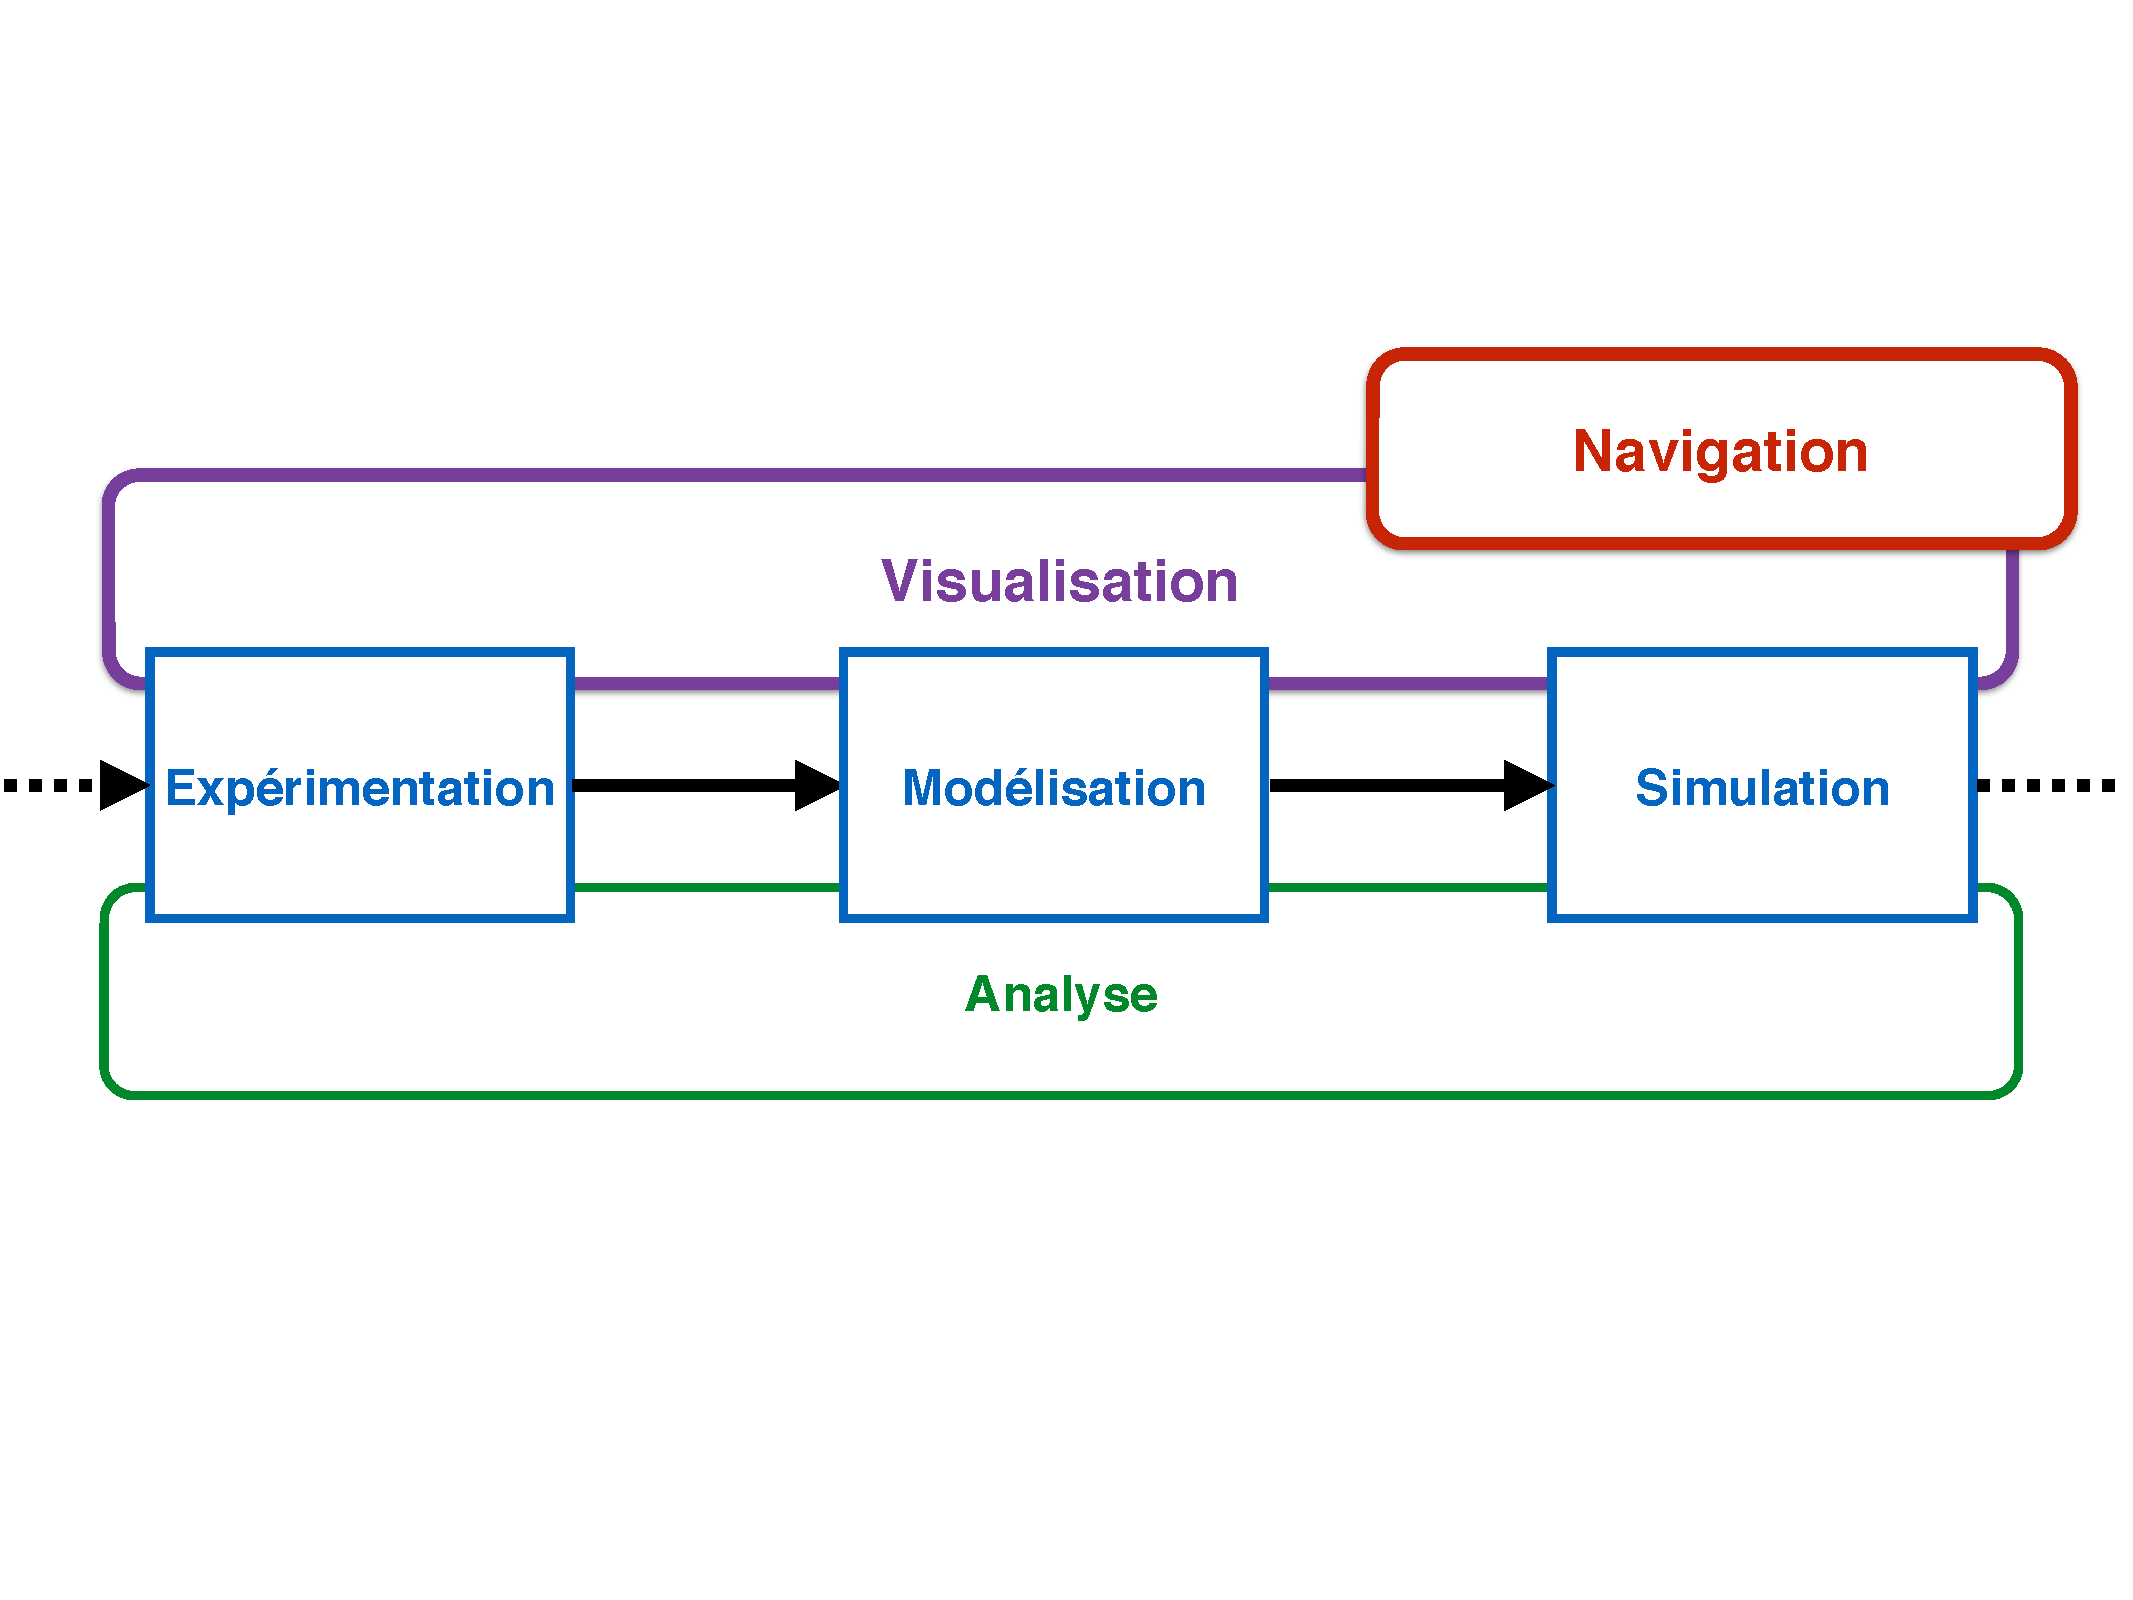
\includegraphics[width=1.0\linewidth]{./figures/ch3/process_bio_struct_navigation}}
    \caption{\it Schéma du processus itératif d'étude d'une structure moléculaire en biologie structurale. Nous nous intéressons ici à l'outil de visualisation et plus spécifiquement à l'une des méthodes qu'elle introduit, la navigation.}
  \label{Fig:process_bio_struct_navigation}
  \hspace{0.3cm}
\end{figure}

\section{Navigation dans des scènes réalistes ou scientifiques}

Nous avons vu dans le chapitre précédent (voir section \ref{navigation}) que la navigation dans des EV immersifs se caractérisait par la volonté d'étendre les capacités d'exploration de mondes virtuels en dépit des limites physiques imposées par les EV immersifs.

\section{Nouveaux paradigmes pour la RV}

Nous avons mis en évidence le besoin de mettre en place des paradigmes de navigation qui répondent aux problématiques posées par la visualisation moléculaire qui met en jeu des objets scientifiques abstraits, de plus en plus complexes, dans des environnements présentant un nombre réduit de repères spatiaux pour l'utilisateur.

Une piste de réflexion étudiée pour faire du processus de navigation un processus intuitif pour l'utilisateur est de le rendre cohérent avec les données qu'il observe. Si la trajectoire suivie par un utilisateur durant son exploration possède des échos dans la nature même de ce qu'il voit, alors nous parvenons à fournir une information pendant que l'utilisateur effectue une simple tâche de navigation. A l'image de ce qui a été fait pour les scènes réalistes, il est donc important de prendre en compte le contenu virtuel à explorer pour mettre en place un paradigme de navigation efficace. De la même façon, la navigation étant le support d'un nombre important de tâches en visualisation moléculaire, il nous a paru important de prendre également en compte l'activité des experts. 

Il nous a donc paru nécessaire et évident d'utiliser à la fois le contenu moléculaire et la tâche des experts pour guider les paradigmes de navigation. Ce travail a pu être fait en collaboration avec des biologistes travaillant sur des exemples concrets de modélisation de phénomènes biologiques précis et utilisant l'outil de la visualisation moléculaire quotidiennement. Il fut également possible de travailler avec des ergonomistes dont les approches d'analyses et de recueil des informations au travers d'entretiens encadrés furent très utiles à l'identification des besoins des experts. Il est en effet important d'associer les experts du domaine aux étapes initiales de conception de paradigmes afin d'éviter un écart trop important entre leurs attentes et le résultat final.
Nous avons finalement, à la fin d'un premier processus de développement logiciel, mis en place un modèle d'évaluation sous la forme d'une décomposition hiérarchique en utilisant la méthodologie de \textit{Hierarchical Task Analysis} (HTA) afin d'évaluer la performance de nos paradigmes de navigation par rapport à une navigation libre \cite{annett2003hierarchical}.

\subsection{Symétrie moléculaire et axes remarquables comme ancrage visuel}

Même si non-exclusif, notre attention fut rapidement portée sur les molécules les plus difficiles à visualiser ou manipuler dans les logiciels de visualisation moléculaire, à savoir les complexes moléculaires de grande taille. Ces complexes moléculaires sont souvent le résultat d'agencements de monomères (chaînes d'acide-aminés répétées) créant des multimères de taille importante et souvent constitués de plusieurs domaines. Les progrès des simulations moléculaires permettent désormais de simuler ces complexes moléculaires au sein de leur environnement, à l'image des protéines transmembranaires et des membranes dans lesquelles elles sont enfouies. Ces systèmes de plusieurs centaines de milliers d'atomes demandent donc une représentation et une navigation adaptées ne modifiant pas leur perception.

\begin{figure}[h]
  \centering
  {\includegraphics[width=.5\linewidth]{./figures/ch3/molecular_symmetries_drawing}}
    \caption{{\it Différents types de symétries retrouvés dans des complexes moléculaires. En haut, GLIC, une protéine transmembranaire composée de 5 monomères avec un axe de symétrie correspondant au centre du pore formé par l'agencement des 5 monomères. Vue du dessus (à gauche) et vue de côté (à droite). En bas à gauche, une capside de virus composée de 4 types de monomères présentant un centre de symétrie superposé au centre de gravité du virus. En bas à droite, enchevêtrement de tubulines agencées autour d'une symétrie hélicoïdale (axiale + translation verticale) formant un microtubule.}}
  \label{Fig:molecular_symmetries_drawing}
  \hspace{0.2cm}
\end{figure}

Ces assemblages moléculaires ont comme point commun la présence quasi systématique d'axes ou de centres de symétrie autour desquels ils sont construits. Or la symétrie est une particularité géométrique pouvant être facilement exploitable pour la mise en place de chemins de navigation optimisés. Mais ce n'est pas le seul avantage. Il est important de noter qu'au-delà de l'avantage conceptuel qu'ont ces symétries, elles possèdent également un rôle primordial dans la fonction même des complexes moléculaires \cite{goodsell_structural_2000}. Plusieurs exemples de d'arrangements symétriques trouvés dans des complexes biologiques sont illustrés dans la Figure \ref{Fig:molecular_symmetries_drawing}.
Ces axes de symétrie, obtenus de façon automatisés ou renseignés manuellement, peuvent donc permettre de définir une orientation fixe de la scène virtuelle moléculaire ainsi qu'être la base de la génération automatique de chemins de navigation. Les guides de navigation ne sont pas limités aux seules protéines symétriques et il est également possible d'identifier des axes principaux d'inertie qui pourront être utilisé de la même manière que les axes de symétrie. Il nous parait enfin important de permettre aux scientifiques de définir eux-mêmes les axes qu'ils considèrent comme important au sein de leurs complexes moléculaires, à l'image des membranes, de pores au sein des protéines ou de formes rectilignes.

\subsection{Contributions pour la représentation spatiale}

L'un des principaux avantages résultant de la réorientation de la scène virtuelle est la possibilité de fusionner l'axe de symétrie d'un complexe et le vecteur \textit{up} de la scène virtuelle. Un schéma rapportant les notions d'orientation à la fois de la scène virtuelle et de la caméra (ou par extension de l'utilisateur puisqu'ils sont considérés comme fusionnés) est fournie dans la Figure \ref{Fig:orientation_camera_EV}. 
Bien que sommaire, ce réarrangement permet de fournir un premier repère spatial fixe à l'utilisateur. Pour qu'il soit considéré comme tel tout au long de l'expérience virtuelle, nous contraignons le complexe moléculaire à garder cette orientation à tout instant. L'utilisateur est ainsi maintenu orienté de façon cohérente par rapport à l'objet d'étude à tout moment. Pour accroître l'apport spatial de cette réorientation, nous avons choisi d'ajouter une \textit{skybox} entourant la protéine. Une skybox est une texture fixe, présente tout autour de la scène virtuelle et jouant de rôle de paysage visuel non interactif. Le choix de la skybox doit respecter un certain nombre de pré-requis afin de remplir complètement son rôle \cite{vinson_design_1999}, ici de permettre à l'utilisateur de s'orienter à tout instant en regardant autour de lui. La skybox sélectionnée doit comporter deux parties supérieures et inférieures distinctes qui correspondrait à la partie haute et la partie basse de la molécule après sa réorientation. Elle peut très bien remplacer un environnement moléculaire (une membrane typiquement)non explicite et absente du modèle 3d observé.

\begin{figure}[h]
  \centering
  {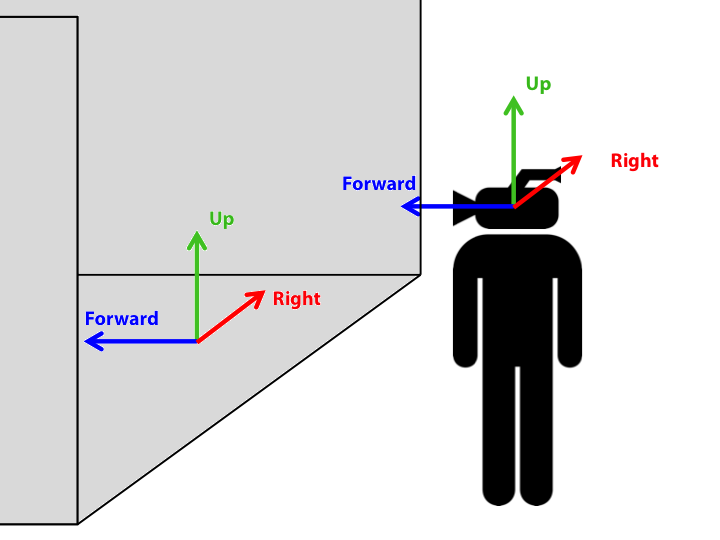
\includegraphics[width=.5\linewidth]{./figures/ch3/orientation_camera_EV}}
    \caption{{\it Schéma de l'orientation dans l'espace de l'utilisateur/camera et de la scène virtuelle (ici dans un système CAVE en gris). L'orientation dans l'espace est représenté par les 3 vecteur up/forward/right.}}
  \label{Fig:orientation_camera_EV}
  \hspace{0.2cm}
\end{figure}

\subsection{Exploration guidée}

De nombreux indices et informations peuvent être récoltés à partir des vues externes d'un complexe moléculaire. Nous savons que la forme générale d'une protéine peut fournir des indices importants sur son état fonctionnel. Nous avons également mis en avant dans la section \ref{visu_molecular} que certaines propriétés physico-chimiques ou géométriques comme la polarité, l'accessibilité au solvant ou l'intégration au sein de l'environnement peuvent être obtenues à partir d'une exploration succinte d'un complexe. Souvent associée au premières étapes de la visualisation, comme énoncé par Shneidermann \cite{shneiderman_eyes_1996}, l'exploration passe par un parcours extérieur du complexe observé. Nous avons mis en place des chemins de navigations circulaires autour de la molécule d'intérêt afin qu'une simple décision de l'utilisateur d'aller à sa droite ou à sa gauche lui permette de tourner autour de la molécule. Cela répond à une première difficulté qui est le suivi d'une trajectoire circulaire lorsque aucune contrainte n'est donnée à l'utilisateur. Il est souvent complexe de gérer des trajectoires circulaires lorsque seuls les axes de translations usuels sont contrôlés par l'utilisateur. Le déplacement latéral est ainsi géré automatiquement de façon à effectuer une rotation axiale autour de l'axe de symétrie, l'utilisateur peut néanmoins contrôler son déplacement vertical et sa distance à la molécule le long respectivement des axes \textit{up} et \textit{forward} de la caméra.

Tout au long du déplacement de l'utilisateur, son orientation est maintenue de façon à avoir le haut de la molécule pointant vers le haut de la scène virtuelle et inversement. Pour ce faire, le vecteur \textit{up} de la caméra est maintenu parallèle au vecteur \textit{up} de la scène. Le maintien de cette orientation est malheureusement préjudiciable lorsque l'utilisateur atteint la hauteur des extrémités hautes et basses du complexe observé. Nous avons donc mis en place un calcul de chemins inspiré de modèle de vecteur global \cite{khan_hovercam:_2005}. Ce modèle de vecteur garde le vecteur \textit{up} coplanaire à l'axe de symétrie et recalcule l'orientation de la caméra (vecteur \textit{forward}) à chaque pas jusqu'à atteindre une perpendicularité entre le vecteur \textit{up} et l'axe de symétrie lorsque l'utilisateur à atteint la hauteur maximale possible (voir Figure \ref{Fig:degree_of_freedom_glic}).

Durant l'étape d'exploration externe l'utilisateur possède donc 3 degrés de liberté en translation même si le déplacement latéral le long du vecteur \textit{right} est contraint pour assurer un mouvement circulaire et le déplacement vertical le long du vecteur \textit{up} est contraint aux extrémités supérieures et inférieures de la protéine afin de garder le focus sur celle-ci. En terme de rotation, le seul degré de liberté autorisé est celui lié au tracking de tête qui verra la caméra suivre la direction du regard de l'utilisateur. Il n'est cependant pas possible de changer l'orientation explicitement pendant l'exploration sous contrainte.

\begin{figure}[h]
  \centering
  {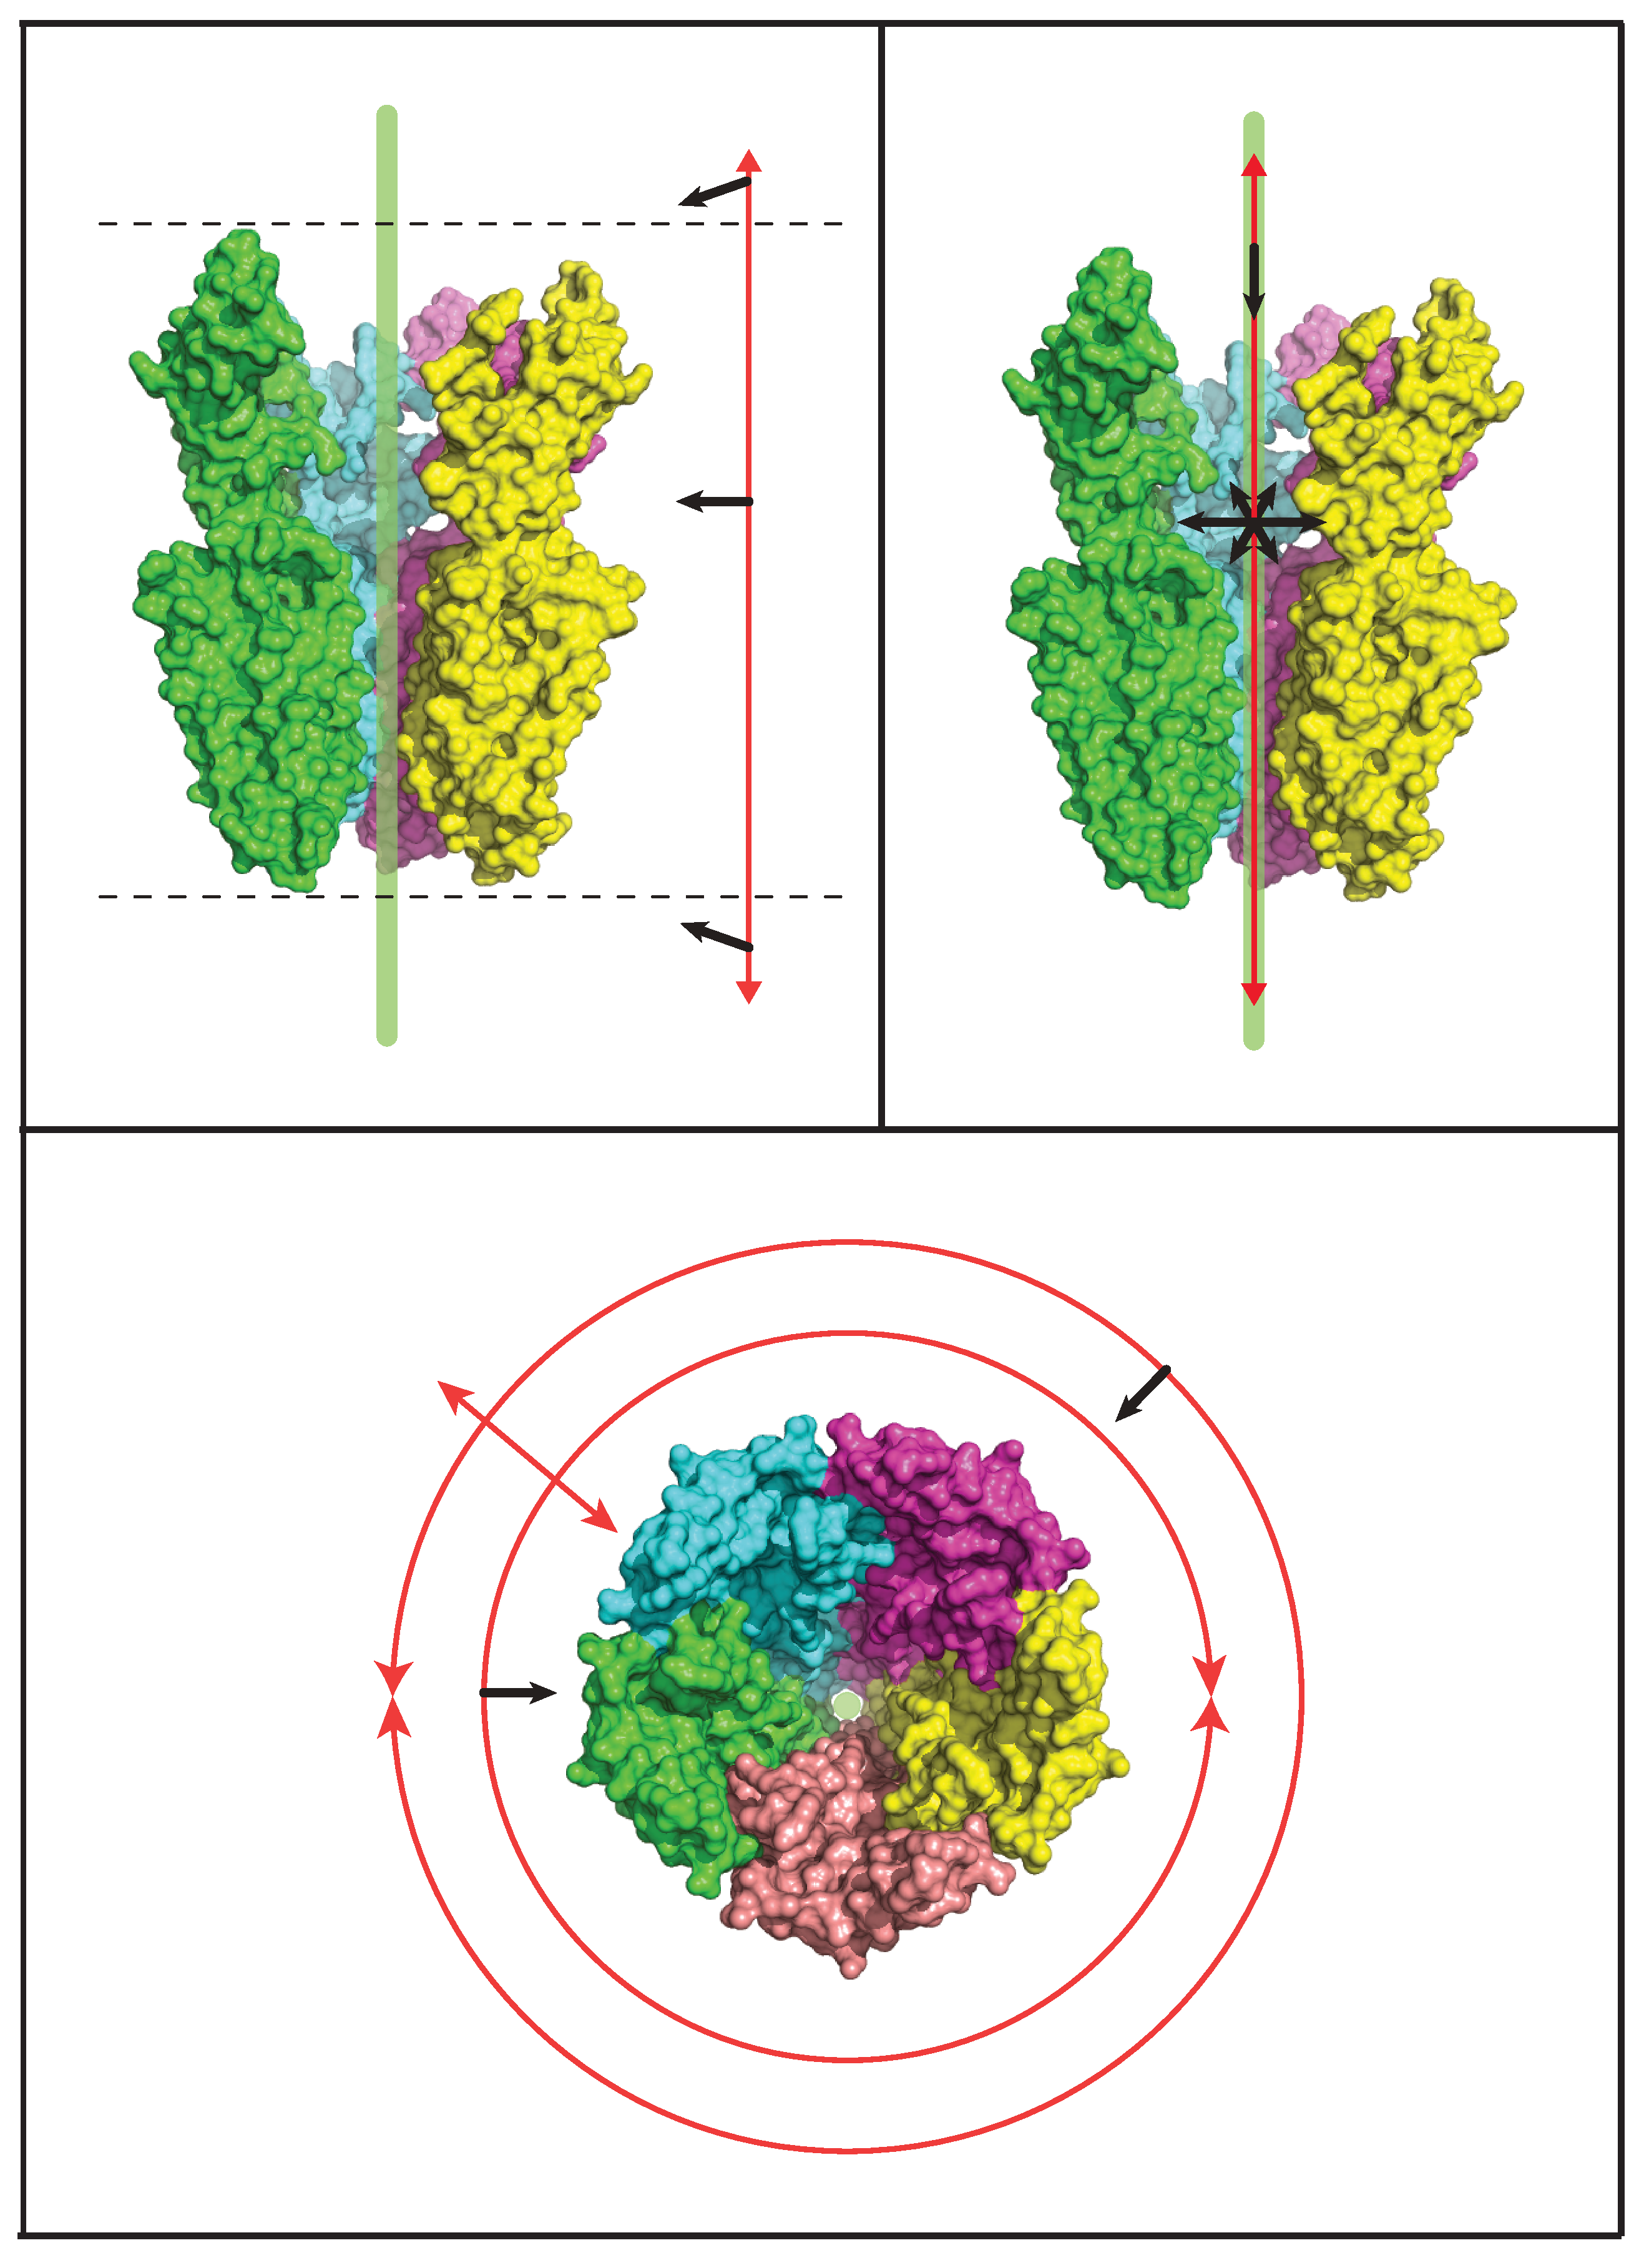
\includegraphics[width=.5\linewidth]{./figures/ch3/degree_of_freedom_glic}}
    \caption{{\it Suivant sa position relative au complexe et dépendant du mode de navigation, la caméra possède un nombre précis de degrés de liberté prédéfinis, à la fois en translation et en rotation. Dans notre illustration, les mouvements de translation possibles sont représentés en rouge alors que les points de vue autorisés sont représentés par des flèches noires. Au cours d'une navigation verticale, la caméra est contrainte sur un axe parallèle à l'axe de symétrie (en vert) quand elle est située à l'extérieur de la protéine (en haut à gauche) ou le long de ce même axe (en haut à droite). Une navigation extérieure contraint le vecteur forward de la caméra pour qu'elle fasse face à la protéine alors qu'à l'intérieur la caméra peut tourner à 360 degrés sur elle-même. Enfin, les chemins de navigation horizontaux à l'extérieur de la protéine (en bas) contraignent le vecteur right de la caméra de façon à ce qu'ils soient circulaires ou perpendiculaires à la protéine pour un effet de zoom avant/arrière.}}
  \label{Fig:degree_of_freedom_glic}
  \hspace{0.2cm}
\end{figure}

La transition entre une exploration interne et externe d'un complexe moléculaire est une question importante qu'il ne semble pas possible de résoudre de façon simple et directe. Certains complexes moléculaires présentent des pores ou des structures centrales ayant un rôle prépondérant dans leur fonction. Parmi ces fonctions, le passage d'ions ou de molécules d'eau ou la liaison avec un ligand sont des phénomènes pouvant prendre place dans des régions enfouies dans un complexe moléculaire. Etant donné leur importance, il était nécessaire de réfléchir à des paradigmes de navigation efficaces dans ces zones d'intérêt tout en gardant la possibilité d'y effectuer des tâches complexes. Dans cette optique, nous avons mis en place la possibilité d'effectuer une transition automatique entre l'extérieur et l'intérieur d'un complexe. A la demande de l'utilisateur, un chemin de navigation rectiligne est calculé pour rejoindre l'intérieur du complexe. Ce chemin part de la position extérieure actuelle de l'utilisateur et rejoint le point de projection de sa position sur l'axe de symétrie de façon à ce que l'axe de symétrie et la trajectoire du chemin créé soient perpendiculaires. 

Lorsque l'intérieur d'une protéine est atteinte, un nouveau set de chemins de navigation est proposé afin de monter ou descendre dans le complexe le long de l'axe de symétrie. Dans ce mode de navigation, un seul degré de liberté en translation est possible ainsi qu'un seul degré de rotation, autour du vecteur \textit{up} de la caméra, comme si l'utilisateur tournait sur lui-même en gardant sa position, comme s'il se trouvait dans un ascenseur panoramique et qu'il dirigeait sa trajectoire verticale. Il est cependant possible d'alterner, pour la translation, vers un déplacement toujours le long de l'axe mais orienté de façon à être face aux extrémités de l'axe de symétrie. A la manière de l'exploration d'un tunnel, ce dernier représentant notre axe de symétrie, l'utilisateur sera capable d'avancer ou de reculer dans ce tunnel. Il pourra de nouveau tourner sur de lui même autour du vecteur \textit{up} de la caméra.

\subsection{Optimisation du parcours des régions répétées}

La symétrie, et plus généralement l'agencement des monomères d'un complexe moléculaire, induit souvent l'apparition d'événements structuraux comme la liaison d'un ligand, l'ouverture d'une poche de liaison ou la simple variation structurelle d'une région de façon répétée pour chaque monomère identique. Ainsi, la liaison d'un ligand sur une première chaîne A signifiera certainement que ce ligand peut aussi se lier à une chaîne identique B, C, D, etc. Comparer ces régions d'intérêts est très utile pour détecter d'éventuels comportements asynchrones ou des effets différents, il peut par contre être difficile de naviguer d'une région à une autre pour effectuer cette comparaison. Grâce à la symétrie, il nous a été possible de mettre en place un mode de navigation adapté à cette problématique permettant d'automatiser complètement le passage d'une région d'intérêt à la région répétée sur un autre monomère. Ce calcul est rendu possible par l'utilisation de l'axe de symétrie comme axe de rotation pour la caméra dont l'angle de rotation sera simplement dépendant de l'angle de rotation ayant été calculé entre les monomères. Un assemblage standard verra cet angle être de 360 degrés divisé par le nombre de monomères identiques du complexe. Il est cependant également possible d'utiliser des scripts de calcul plus fins afin d'obtenir les valeurs d'angle précises entre les monomères impliqués. Lorsque cette information est connue (elle est par défaut calculée lors de la phase d'initialisation de la scène virtuelle) et que l'utilisateur a choisi son point de vue sur la région d'intérêt, alors une simple interaction avec un bouton permet de parcourir les différents monomères, préservant le point de vue choisi initialement. Il est possible de parcourir les monomères dans les deux sens. Chaque déplacement est effectué automatiquement et une série d'interpolations au cours de la trajectoire de la caméra permet une transition douce entre les différentes positions.

\subsection{Trouver un point de vue optimal}

Même si l'exploration peut apporter un grand nombre d'informations, certains phénomènes moléculaires ne concerne qu'une poignée d'atomes ou de résidus. Au sein de large structures de plusieurs millions d'atomes, ces zones d'intérêt deviennent difficiles à visualiser à cause de la densité des particules voisines. De plus, certaines régions sont profondément enfouies dans le complexe moléculaire, transformant la simple tâche de visualisation en un défi pour l'utilisateur. Afin de résoudre cette problématique, nous avons développé un algorithme capable de calculer le meilleur point de vue pour la caméra, connaissant les coordonnées de la cible et la distance à laquelle la caméra devra être située. Cet algorithme prend en compte les atomes entourant la cible et calcule les cônes de vue les plus larges pour identifier le meilleur point de vue. L'utilisateur aura la possibilité de choisir entre plusieurs cônes de vue afin d'obtenir un angle de vue différent sur la cible choisie.

\begin{figure}[h]
  \centering
  {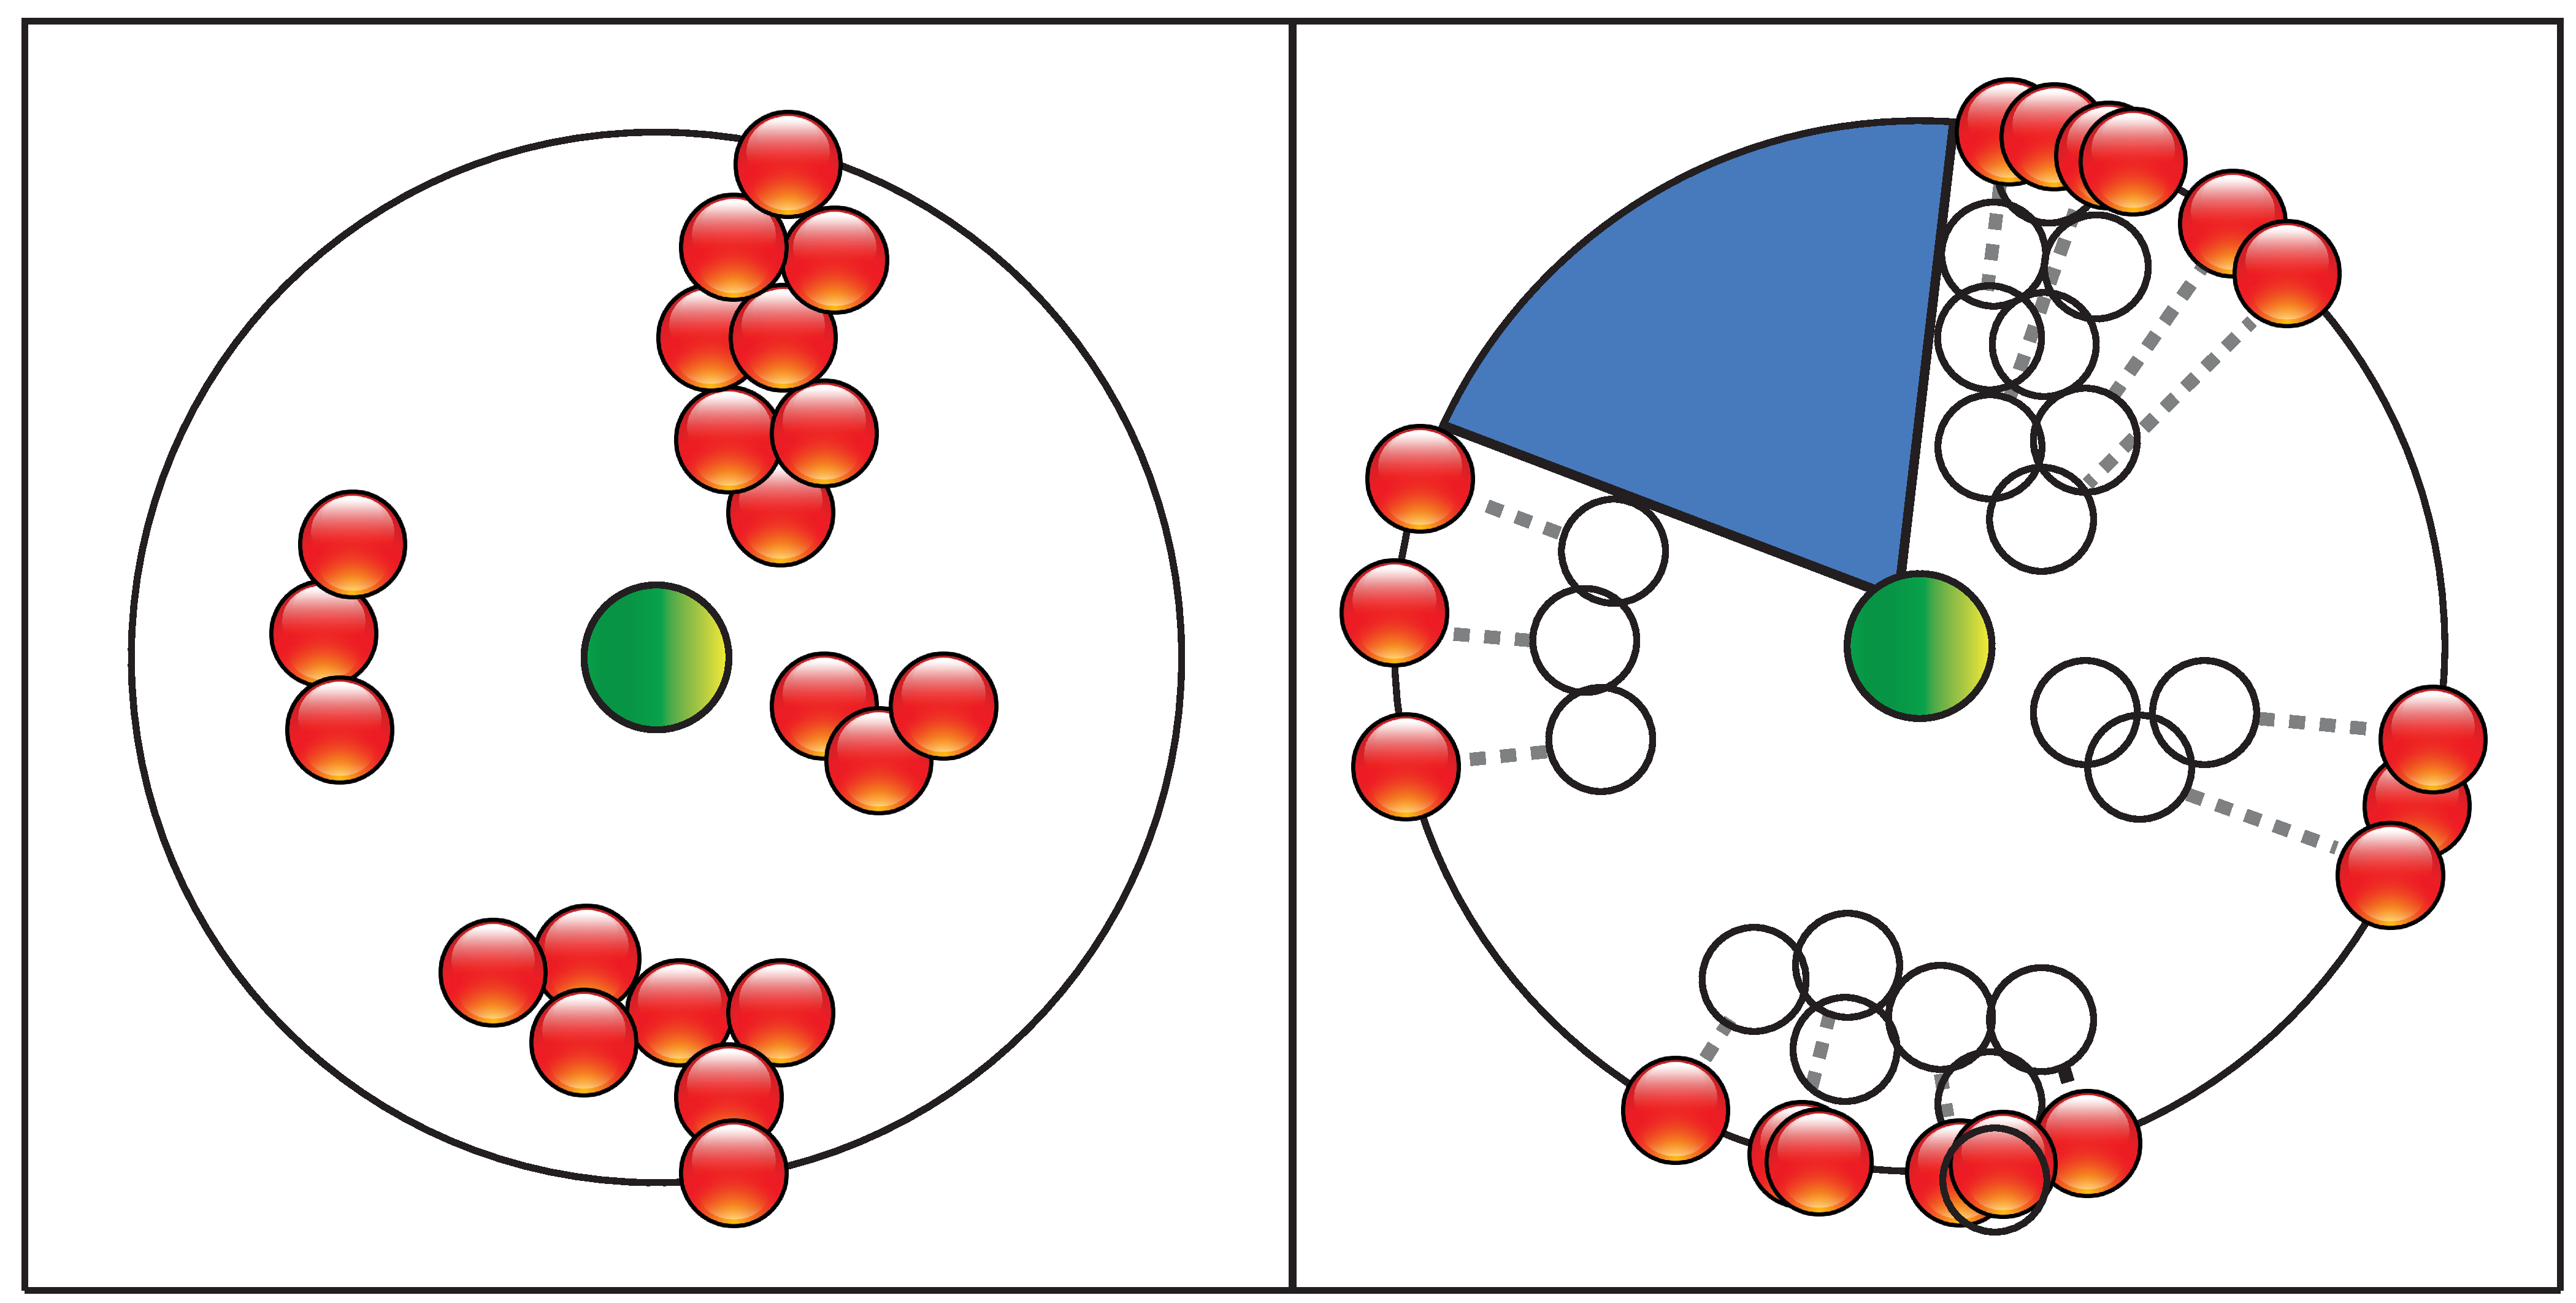
\includegraphics[width=.5\linewidth]{./figures/ch3/voronoi_2D_algo_v2}}
    \caption{{\it Schéma de l'étape 3 de l'algorithme de point de vue optimal, représenté en 2d. A gauche, notre cible est représentée en vert, ses atomes voisins en rouge et le cercle représente la distance à laquelle l'utilisateur veut placer sa caméra. A droite, les atomes voisins sont projetés sur le cerle et on cherche la portion de ce cerle possédant le plus large espace vide afin d'obtenir le cône de vue le plus large représenté en bleu.}}
  \label{Fig:voronoi_2D_algo}
  \hspace{0.2cm}
\end{figure}

\subsubsection{Algorithme}

L'algorithme utilisé pour obtenir les cônes de vue peut être décomposé de la sorte:

\begin{enumerate}
	\item L'utilisateur fournit les coordonnées 3d de la cible soit en entrant les valeurs (x,y,z) au sein d'une fenêtre de saisie, soit via une sélection directe. Si la cible comporte plus d'un atome alors les coordonnées du centre de masse de la sélection seront calculées. La hauteur désirée du cône de vue \textit{d} est également demandée, elle correspondra à la distance de la caméra par rapport à la cible.
	\item Tous les atomes situés au sein d'une sphère de rayon \textit{d} et centré sur les coordonnées de la cible sont considérés comme voisins et comme potentielles occlusions, ou obstacles, pour le cône de vue. Leurs coordonnées 3d sont stockées.
	\item L'ensemble des coordonnées 3d des atomes voisins stockés précédemment sont décalés dans l'espace d'un vecteur correspondant aux coordonnées 3d de la cible (un cible située en $(1.2,-9.2,5.5)$ entraînera un décalage des coordonnées de $\overrightarrow{(1.2,-9.2,5.5)}$). Cela entraîne la création d'une sphère dont les coordonnées d'atomes sont centrées autour d'une origine (la cible) située en $(0,0,0)$.
	\item L'ensemble des coordonnées cartésiennes des atomes contenus dans la sphère sont transformées en coordonnées sphériques. Les coordonnées sphériques sont composées de 3 paramètres: une distance radiale à l'origine \textit{r}, un angle polaire $\theta$ (theta) et un azimuth $\phi$ (phi). En mettant de côté la distance radiale, nous obtenons pour chaque atome une information de direction par rapport à l'origine donnée par les angles $\theta$ et $\phi$. Il est possible de fixer la distance radiale de tous les atomes voisins à la valeur de \textit{d} et ainsi mettre en place une projection de ces atomes sur la sphère de rayon \textit{d}. Lorsque la projection est effectuée, la recherche du plus large cône de vue passera par la recherche du plus grand cercle vide à la surface de la sphère. Le concept est illustré dans la Figure \ref{Fig:voronoi_2D_algo}
	\item Puisque la valeur de la distance radiale est identique pour l'ensemble des atomes voisins, il est possible de créer un nuage de point correspondant aux valeurs de $\phi$ en fonction des valeurs des valeurs de $\theta$ afin d'obtenir une représentation aplatie de la surface de la sphère en 2d contenant l'ensemble des points projetés (un point = un atome). La matrice 2d ainsi obtenue est étendue de 50\% le long des ordonnées et des abscisses afin de prendre en compte la périodicité de la sphère. Il n'est pas nécessaire de l'étendre au-delà de 50\% puisque la taille maximum d'un cercle vide sera la taille du plus long côté de la matrice. Si aucune extension n'est effectuée, nous pourrions manquer les solutions qui apparaîtraient à l'extrémité de la matrice où deux régions de la sphère aplatie se rejoindraient. Nous pouvons d'ailleurs voir dans la Figure \ref{Fig:voronoi_diagram} que l'absence d'extensions nous auraient fait manquer deux solutions. Pour synthétiser, ces nuages de points 2d peuvent être considérés comme une carte 2d de la distribution à la surface de la sphère des atomes ayant été projetés.
	\item A partir de la liste des atomes formés par les paires $\theta$/$\phi$, un diagramme de Voronoi est calculé. Nous obtenons une liste de sommets de Voronoi associés chacun à un triplet des trois atomes les plus proches.
	\item La distance entre chaque sommet de Voronoi et les trois points les plus proches est calculée et les plus grandes valeurs de cette distance indiquera les plus grands cercles vides présents sur la surface de la sphère. Ces cercles auront pour centre un sommet de Voronoi et passeront obligatoirement par les trois points les plus proches puisque l'algorithme de Voronoi impose que chaque sommet soit équidistant d'au moins 3 points, ceux-ci étant également les plus proches. Le cercle avec le rayon le plus large sera considéré comme le cercle vide le plus grand (cf. Figure \ref{Fig:voronoi_diagram}). Il est important de noter que, en dépit de l'extension de la matrice, nous ne sélectionnons pas de centres de cercles situés à l'extérieur de la boîte entourant les premières coordonnées sphériques tracées (en pointillé dans la Figure \ref{Fig:voronoi_diagram}) et correspondant aux extensions. Cependant les points appartenant au cercle peuvent eux se situer dans les parties étendues du graphe.
	\item Les valeurs $\theta$/$\phi$ du centre des plus larges cercles vides sont transformés en coordonnées cartésiennes et décalés de nouveau d'un vecteur opposé à celui utilisé pour le premier décalage (avec notre exemple ce vecteur serait $\overrightarrow{(-1.2,9.2,-5.5)}$). Le rayon des cercles donne un angle d'ouverture qui sera utilisé par la suite pour calculé une trajectoire optimale (voir ci-dessous).
	\item Les coordonnées cartésiennes peuvent ensuite être choisies itérativement par l'utilisateur pour se positionner par rapport à la cible, la caméra sera contrainte de façon à toujours faire face à la cible.
\end{enumerate}

Cet algorithme a une complexité faible en $\theta(n.\log{n})$ (avec $n$ désignant le nombre d'atomes) puisque la recherche des voisins de la cible est calculée en $n$-1 itérations (constant) et que le diagramme de Voronoi et la recherche du cercle le plus large est effectué en $\theta(n.\log{n})$ dans le pire des cas où tous les atomes du système sont considérés comme voisins et situés dans la sphère de rayon \textit{d}. L'algorithme est capable de fournir une liste des vues les plus dégagées sur une cible de façon quasi instantanée et donc permet à l'utilisateur de changer de point de vue rapidement.

\begin{figure}[h]
  \centering
  {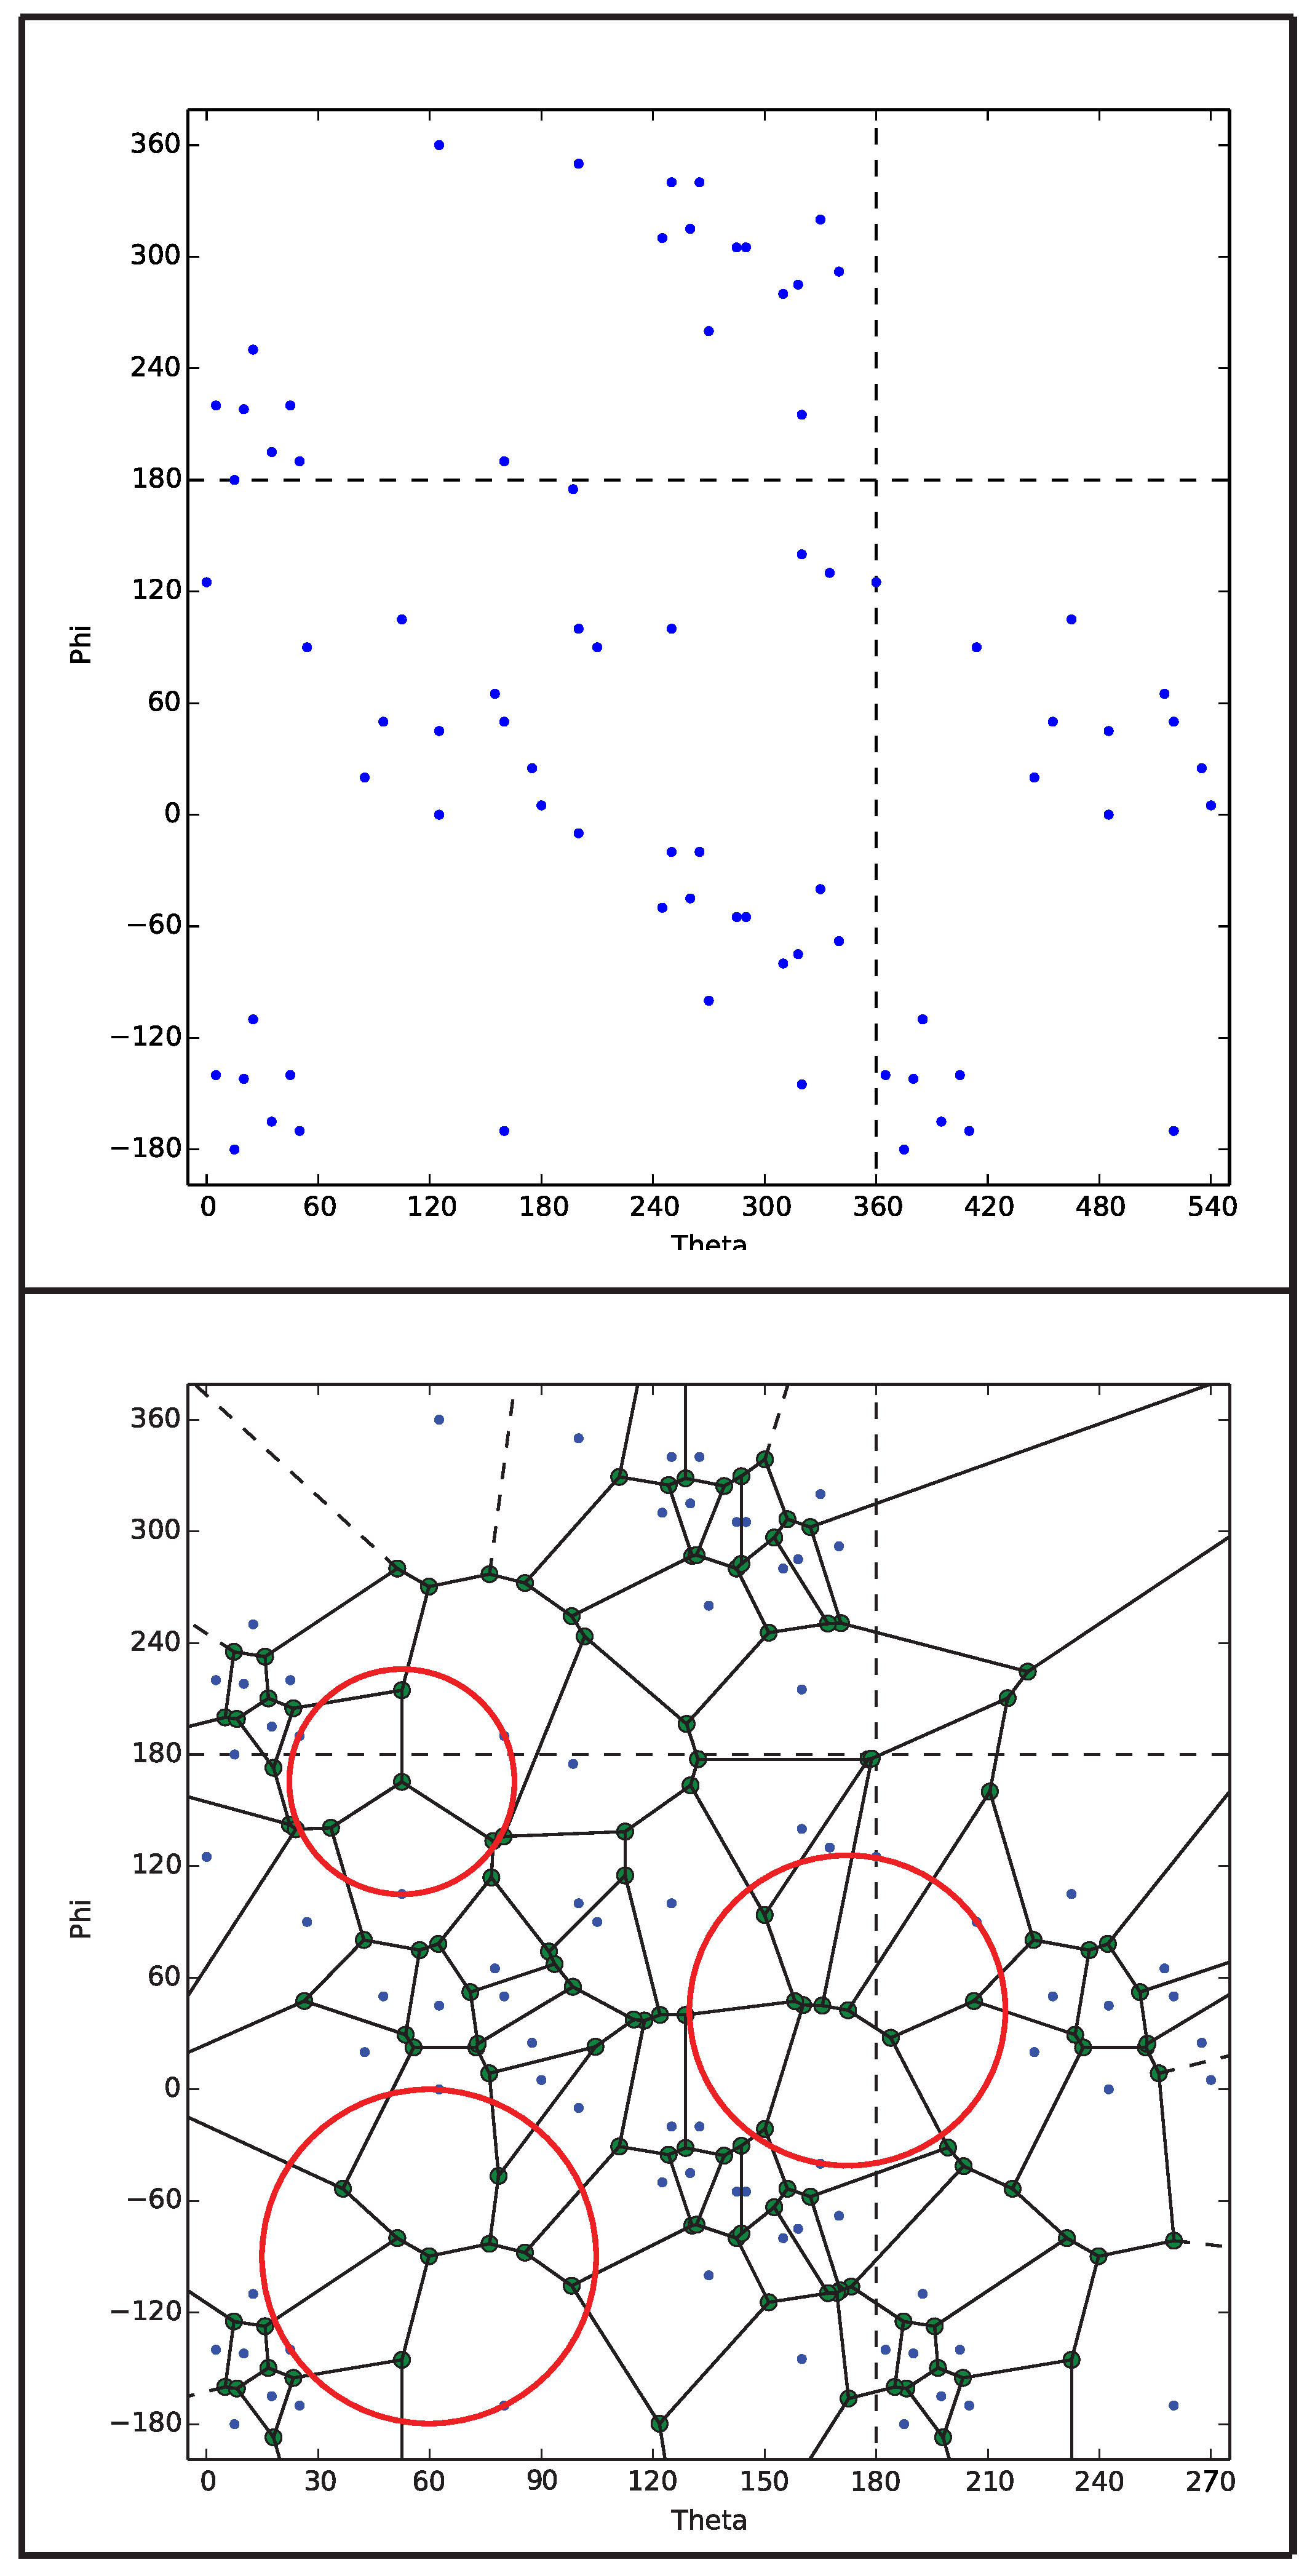
\includegraphics[width=.5\linewidth]{./figures/ch3/voronoi_diagram}}
    \caption{{\it En haut, graphique représentant les angles $\phi$ en fonction des angles $\theta$ des atomes voisins de la cible, chaque atome est représenté par un point bleu. En bas, même graphique contenant en plus les sommets (en vert) et les segments (lignes noirs) du diagramme de Voronoi ayant été calculé sur les coordonnées sphériques des atomes voisins (en bleu). Les cercles rouges représentent les plus larges cercles vides pouvant être trouvés au sein des points bleus.}}
  \label{Fig:voronoi_diagram}
  \hspace{0.2cm}
\end{figure}

\subsubsection{Atteindre les points de vue optimaux}

La recherche d'un point de vue optimal peut être effectuée sur n'importe quelle région du complexe moléculaire étudié, nous avons cependant mis en avant son apport dans le cas de régions d'intérêt à observer enfouies dans le complexe et très difficilement atteignables. Le chemin entre la position d'un utilisateur au moment où il décide de rentrer dans un mode de recherche de point de vue optimal et la position optimale trouvée passe souvent par le passage au travers du complexe, dans des régions potentiellement denses en atomes et perturbantes pour le point de vue de l'utilisateur. Il nous a donc paru nécessaire de mettre en application les recommandations énoncées dans la section \ref{cybersickness} qui rappelaient l'importance des transitions entre points de vue pour diriger une trajectoire entre deux points d'une scène virtuelle. Afin tout d'abord de minimiser l'impact négatif que pourrait avoir ce déplacement sur l'utilisateur et ensuite pour permettre à l'utilisateur de garder une conscience spatiale de l'environnement pendant le déplacement et ainsi pouvoir se situer rapidement lors de son positionnement final devant la cible visée.
Une transition progressive et automatique est ainsi mise en place. Pour calculer les différents points du chemin reliant la position initiale de l'utilisateur à la position optimale de visualisation de sa cible, l'algorithme développé précédemment est utilisé de façon répété à différentes valeurs de \textit{d} et appliqué à une aire restreinte de la surface de la sphère correspondant aux aires délimitées par les cercles vides identifiés lors de la première itération de l'algorithme. Comme illustré dans la Figure \ref{Fig:optimal_pov_camera_path} nous obtenons un chemin de navigation avec le moins d'occlusions pendant la majorité de la phase d'approche de la position optimale.

\begin{figure}[h]
  \centering
  {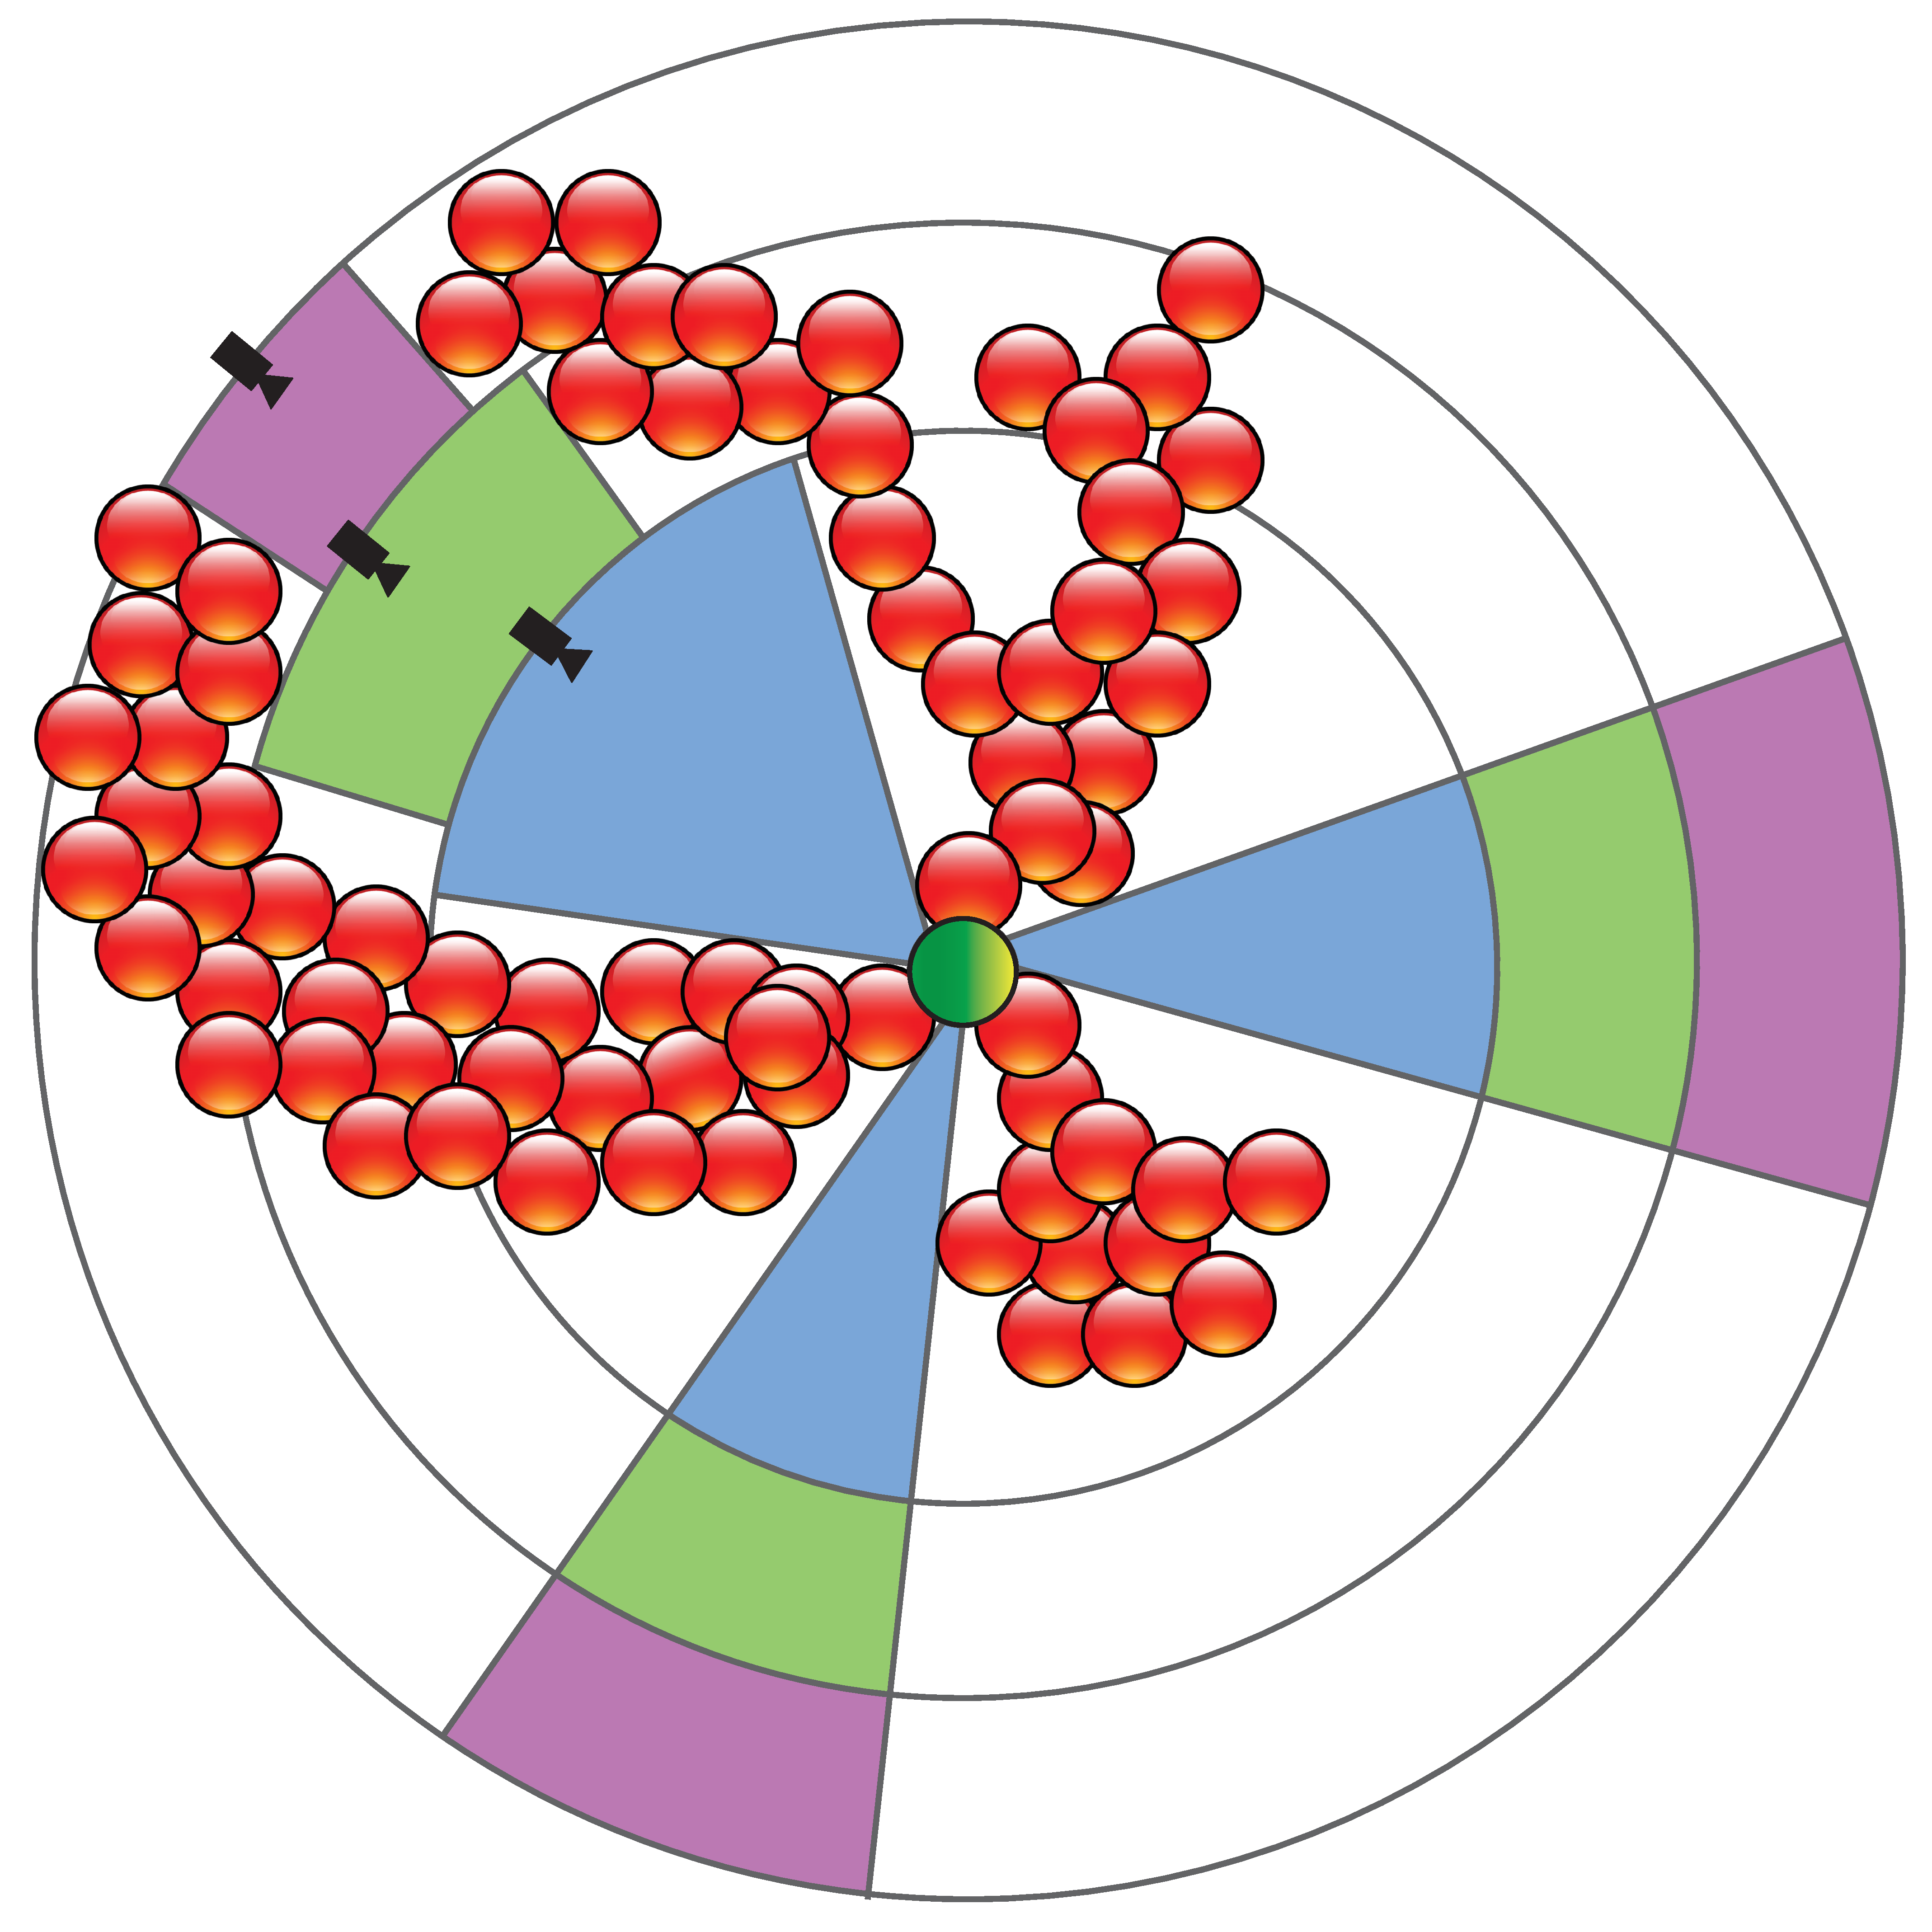
\includegraphics[width=.5\linewidth]{./figures/ch3/optimal_pov_camera_path}}
    \caption{{\it Schéma de l'algorithme de recherche du meilleur chemin de caméra pour atteindre un point de vue optimal. La cible à visualiser est représentée en vert et ses atomes voisins en rouge. Chaque cercle représente une distance précise entre la caméra et la cible, le cercle le plus petit désignant la distance désirée par l'utilisateur. Pour chaque distance, l'algorithme de point de vue optimal est utilisé afin d'obtenir les meilleurs point de vue sur la cible. Les cônes bleus représentent les cônes de vue les plus larges trouvés alors qu'en vert et violet sont représentés les aires vides les plus larges entre les différentes distances de caméra. Le chemin qu'empruntera la caméra pour atteindre le point de vue optimal est ainsi représenté grâce aux symboles de couleur noire. Ce chemin est calculé pour garder un point de vue le plus dégagé possible jusqu'à atteindre le point final.}}
  \label{Fig:optimal_pov_camera_path}
  \hspace{0.2cm}
\end{figure}

Cela permet également de laisser à l'utilisateur la possibilité de choisir entre la position offrant le plus large cône de vue sur la cible ou la position dont le chemin d'accès est le plus dégagé parmi les positions optimales recensées. Selon la distance entre la position initiale de l'utilisateur et les positions optimales identifiées, la première partie de la trajectoire peut être calculé comme une ligne droite afin de réduire le nombre d'itérations de l'algorithme, ce dernier demandant en plus un temps de calcul augmentant à chaque pas de temps à cause de la taille de la sphère créée et du nombre de voisins considérés.

Le passage d'un point de vue optimal à un autre est quant à lui simplement le fruit de techniques d'interpolation classiques prenant en compte la préservation du focus sur la cible, la recherche d'une orientation de la caméra dont le vecteur \textit{up} est le plus parallèle possible de l'axe de symétrie et le chemin le plus court pour atteindre la nouvelle position.

\subsubsection{Grande densité atomique}

Dans le cas de régions très denses et d'une cible particulièrement enfouie dans ces régions, nous avons ajouté la possibilité de rendre transparents les atomes situés entre la caméra et la cible. Ce traitement graphique n'est pas effectué dans l'intégralité de l'écran mais seulement dans un cercle de taille fixe centré sur le centre de l'écran. Cela permet de supprimer toute occlusion le long du déplacement pour atteindre le point de vue optimal désiré.

Dans le cas où l'algorithme de point de vue optimal n'est pas suffisant pour permettre la visualisation d'une cible sans occlusions devant la caméra, nous avons mis en place une étape supplémentaire dans le processus de visualisation. Cette étape est une étape de modification structurelle du complexe moléculaire. Elle consiste à découper le complexe moléculaire en sous-régions distinctes et de permettre leur dissociation pendant l'exploration. Ce découpage ne peut cependant pas se faire de façon simpliste et demande une définition intelligente des sous-régions afin de ne pas perdre toute cohérence structurale et donc biologique du complexe moléculaire. Nous avons de nouveau utilisé la géométrie du complexe moléculaire comme base de décision pour ce découpage. Puisque la symétrie définie les monomères d'un complexe, nous pouvons facilement découper la structure pour que ces monomères puisse bouger de façon contrôlée et de manière à ne pas perdre la forme générale de la structure (voir Figure \ref{Fig:fragmented_view}). L'utilisateur a de plus la possibilité, à chaque instant, d'étendre, rétrécir ou simplement déplacer les monomères du complexe en fonction de l'axe ou du centre de symétrie qu'il choisit (dans le cas où plusieurs axes/centres ont été renseignés). Un mode automatisé a également été ajouté permettant d'étendre ou rétrécir la structure suivant la position de l'utilisateur par rapport au complexe. Une distance maximum d'extension peut être imposée afin de préserver les informations d'interaction entre les monomères ou les sous-unités découpées. Cette adaptation structurelle permet la mise en lumière des interfaces enfouies entre les sous-unités et permettre de calculer de nouveaux points de vue optimaux. Pour éviter toute surcharge dans le processus de modification structurelle, la configuration spatiale initiale du complexe peut être retrouvée à chaque instant.

\begin{figure}[h]
  \centering
  {\includegraphics[width=.5\linewidth]{./figures/ch3/fragmented_view}}
    \caption{{\it Dessin illustratif d'une protéine présentant un pore central constituant son axe de symétrie. A gauche, les monomères du complexe moléculaires sont écartées de l'axe de symétrie. Au centre, différentes région d'intérêt ont été identifiées le long des monomères et le complexe est écarté de façon verticale. A droite sont combinés la séparation des monomères et des régions d'intérêt. Illustration de Davide Spalvieri.}}
  \label{Fig:fragmented_view}
  \hspace{0.2cm}
\end{figure}


\subsubsection{Evaluation par Analyse Hiérarchique de la Tâche (HTA)}

Nous avons choisi d'évaluer nos paradigmes de navigation au moyen de la décomposition hiérarchique de deux tâches identifiées comme habituelles pour les experts scientifiques. Le choix de ces tâches a pu se faire grâce à la contribution d'ergonomes et au moyen de méthodes d'entretiens supervisés.
Nous sommes partis du constat que l'évaluation systématique de tâches métier est impossible ou très difficile à cause de plusieurs facteurs: (1) la spécialisation de l'outil évalué est très importante et nous faisons face à un outil dont la nature (PyMol, VMD, Yasara) varie suivant les usages usuels des experts scientifiques interrogés. (2) L'implémentation et l'adaptation de nos paradigmes sur un ensemble représentatif d'outils spécialisés est compliquée et très chronophage. (3) Notre démarche est biaisée de part son développement basé sur l'exécution de tâches expertes. L'utilisation de tâches expertes pour l'évaluation d'une approche basée sur ces tâches nous parait litigieuse. 

Nous proposons donc dans cette partie l'emploi d'une méthode d'évaluation plus théorique qu'empirique pour cerner l'efficacité de notre approche. La méthode HTA consiste en une subdivision d'une tâche principale en plusieurs sous-tâches précises. Chaque sous-tâche peut à son tour être subdivisée jusqu'à ce que les sous-tâches atteignent un degré de précision suffisant pour qu'il soit possible de donner une approximation du temps d'exécution qu'elle nécessite pour être accomplies.

C'est une méthode très usitée par les ergonomistes qui la dédient à plusieurs fins dont l'optimisation de tâches, la conception d'interfaces, etc.


L'arbre de tâche HTA présenté ci-dessous décrit la manière de répondre à une tâche courante de visualisation moléculaire, la recherche d'un ligand au sein d'un complexe moléculaire. Nous utiliserons l'exemple de la liaison du bromoforme avec GLIC pour illustrer cet exemple. Ce modèle, extrait grâce aux experts du domaine, donne une subdivision progressive de la tâche énoncée. Les subdivisions les plus externes pouvant finalement être évaluées d'un point de vue temporel. Nous comparons ici des conditions de navigation libres avec des conditions de navigation guidée utilisant les paradigmes expliqués précédemment. Nous ferons l'hypothèse d'une situation initiale identique dans le même logiciel de visualisation moléculaire pour les deux conditions évaluées.
\\
\\
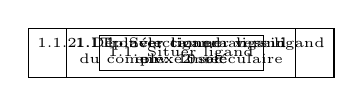
\begin{tikzpicture}
\tikzset{grow'=right,level distance=120pt}
\tikzset{execute at begin node=\strut}
\tikzset{every tree node/.style={anchor=base west}}
\Tree 
 [.\node[draw, font=\tiny, align=center]{1. Trouver ligand au sein\\ du complexe moléculaire};
    [.\node[draw, font=\tiny, align=center]{1.1. Situer ligand} ;
        [.\node[draw, font=\tiny, align=center](start){1.1.1. Sélectionner ligand \\env. 2 sec}; ]
        [.\node[draw, font=\tiny, align=center]{1.1.2. Déplacer camera vers ligand \\env. 10 sec}; ] ]
 ] 
    \\           
\end{tikzpicture}
\\
\\
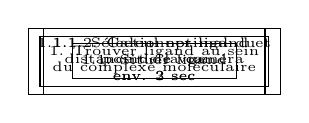
\begin{tikzpicture}
\tikzset{grow'=right,level distance=150pt}
\tikzset{execute at begin node=\strut}
\tikzset{every tree node/.style={anchor=base west}}
\Tree 
 [.\node[draw, font=\tiny, align=center]{1. Trouver ligand au sein\\ du complexe moléculaire};
    [.\node[draw, font=\tiny, align=center]{1.1. Situer ligand} ;
        [.\node[draw, font=\tiny, align=center]{1.1.1. Sélectionner ligand et\\ distance de la caméra \\env. 3 sec}; ]
        [.\node[draw, font=\tiny, align=center]{1.1.2. Calcul optimal du\\ point de vue \\ env. 2 sec}; ] ]
 ] \\           
\end{tikzpicture}
\\

Cette première tâche peut être considérée comme simple et ne comporte après sa décomposition en sous-divisions que deux étapes. Tout d'abord la sélection du ligand pour le mettre en avant au sein de la scène moléculaire puis le déplacement de la caméra pour une vision rapprochée sur sa position et son environnement proche. Alors que cette tâche prendre environ 12 secondes lors d'une session de navigation sans contraintes, elle est réduite à 4 secondes avec les paradigmes de navigation mis à disposition. L'algorithme de point de vue optimal est particulièrement utile ici puisqu'il permet, grâce à la sélection du ligand et une distance de caméra émise par l'utilisateur, de calculer automatiquement le meilleur point de vue sur le ligand ainsi que le chemin optimal pour y accéder.

Nous avons identifié une seconde tâche métier type, dans la continuité de la première, et consistant à identifier, au sein d'un complexe protéique multimérique composé de 5 monomères, les différents acides aminés impliqués dans la liaison avec le ligand identifier précédemment. Cette identification des résidus en contact avec le ligand devra être effectuée pour chaque monomère du complexe. Cette tâche est divisible en deux étapes principales: L'identification des résidus en interaction et l'accès au monomère suivant. Suivant les conditions d'expérience initiales, la subdivision de chacune de ces deux étapes est différente et décrite dans les deux arbres hiérarchiques suivants. On obtient un temps d’exécution pour cette tâche plus élevé dans les conditions normales (environ 2 min 12 s) que dans les conditions intégrant nos paradigmes de navigation (environ 1 min 8 s). L'accès à la cible (ici le ligand) et la recherche du monomère suivant sont les deux étapes cruciales où les paradigmes de navigation permettent un gain de temps substantiel. De façon moins tangible car difficilement mesurable, nos paradigmes permettent également d'assurer une vision sans occultations de la zone cible et donc pourrait être considéré comme facilitant l'étape 2.2.
\\
\\
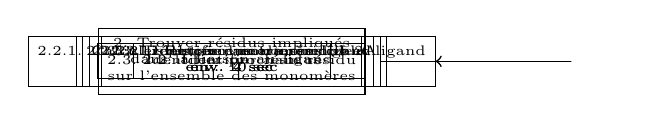
\begin{tikzpicture}
\tikzset{grow'=right,level distance=120pt}
\tikzset{execute at begin node=\strut}
\tikzset{every tree node/.style={anchor=base west}}
\Tree 
 [.\node[draw, font=\tiny, align=center]{2. Trouver résidus impliqués \\dans la liaison au ligand \\sur l'ensemble des monomères};
    [.\node[draw, font=\tiny, align=center]{2.2. Identifier résidus} ;
        [.\node[draw, font=\tiny, align=center](start){2.2.1. Calculer distance entre résidus et ligand \\env. 10 sec}; ]
        [.\node[draw, font=\tiny, align=center]{2.2.2. Lister résidus a moins de 2A \\env. 2 sec}; ] ]
    [.\node[draw, font=\tiny, align=center]{2.3. Identifier prochain résidu};
    	[.\node[draw, font=\tiny, align=center]{2.3.1. Retour vue d'ensemble \\env. 4 sec}; ]
    	[.\node[draw, font=\tiny, align=center]{2.3.2. Identifier monomère cible \\env. 4 sec}; ] 
    	[.\node[draw, font=\tiny, align=center](end){2.3.3. Déplacer caméra sur ligand \\env. 10 sec}; ] ] 
    ] 
 \draw[semithick,->] (end)..controls +(east:5) and +(east:5)..(start);
    \\           
\end{tikzpicture}
\\
\\
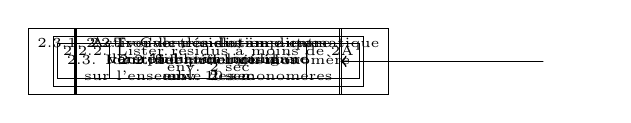
\begin{tikzpicture}
\tikzset{grow'=right,level distance=150pt}
\tikzset{execute at begin node=\strut}
\tikzset{every tree node/.style={anchor=base west}}
\Tree 
 [.\node[draw, font=\tiny, align=center]{2. Trouver résidus impliques \\dans la liaison au ligand \\sur l'ensemble des monomeres};
    [.\node[draw, font=\tiny, align=center]{2.2. Identifier résidus} ;
        [.\node[draw, font=\tiny, align=center](start){2.2.1. Calculer distance entre \\résidus et ligand \\ env. 10 sec}; ]
        [.\node[draw, font=\tiny, align=center]{2.2.2. Lister résidus à moins de 2A \\ env. 2 sec}; ] ]
    [.\node[draw, font=\tiny, align=center]{2.3. Identifier prochain monomère};
    	[.\node[draw, font=\tiny, align=center](end){2.3.1. Activer la translation automatique \\ vers prochain monomère \\ env. 2 sec}; ] ] 
 ] 
\draw[semithick,->] (end)..controls +(east:5) and +(east:5)..(start);
    	\\           
\end{tikzpicture}
\\

\subsection{Conclusion}

La visualisation de données est un processus analytique où l'observation et l'exploration des données amènent de nouvelles informations au scientifique. Cette information peut être acquise d'une façon active, en mesurant par exemple la distance entre deux atomes, ou de façon passive, en se déplaçant et en observant des phénomènes qui ne peuvent être que partiellement décrits par des valeurs brutes. C'est le cas par exemple de la forme des surfaces situées à l'interface entre deux partenaires biologiques se liant entre-eux qui ne peuvent être définis que de manière parcellaire par des propriétés d'hydrophobicité, d'accessibilité au solvant ou de volume et qui nécessitent donc d'être visualisés afin d'être totalement comprises. L'acquisition d'informations passe donc par un processus de navigation qui dirige l'utilisateur vers les événements qu'il désire observer ou vers des régions avec lesquelles il désire interagir. La navigation est un processus important en immersion car il peut décider du confort de l'utilisateur pour effectuer ses tâches, passives ou actives. Le malaise du virtuel, lié en partie à la perte de repères spatiaux est un phénomène qu'il est important de prendre en compte mais qui fut absent des approches de navigation, et  plus précisément de manipulation, développées avec les logiciels experts de visualisation moléculaire. Cette absence est principalement due à l'aspect négligeable du cybersickness en conditions non-immersives.

Fort du constat de l'absence de développements de navigation spécifiques à la visualisation de données scientifiques et plus particulièrement moléculaires, nous avons proposé plusieurs paradigmes ou modes de navigation pouvant répondre à ce besoin. Nos efforts se sont portés sur l'utilisation de l'objet d'intérêt, ici un complexe moléculaire, comme base intelligente et dynamique de la créations de chemins de navigation contraints, semi-automatisés ou automatisés suivant les modes de navigation considérés. Notre approche peut s'inscrire dans le processus de visualisation de données évoqué par Shneidermann et introduisant une échelle de granularité partant de l'exploration globale des données à l'observation précise de certains phénomènes ponctuels et locaux.

Nos développements se sont basés sur le contenu et la tâche mais se sont voulus indépendants de toute considération de contexte et nos paradigmes peuvent être utilisés sur n'importe quelle plateforme et sont complètement indépendants des périphériques d'interaction utilisés. Cette généricité permet un utilisation à la fois au sein d'EV immersifs mais également de stations de travail fixes.

La généricité de notre approche peut également être soulignée par le nombre d'applications potentielles auxquelles elle peut répondre. En effet, les applications venant de domaines où la visualisation de données abstraites présentant une densité importante d'informations pourrait bénéficier de notre étude. La mécanique des fluides, les sciences des matériaux, la climatologie, la médecine ou l'astronomie sont des exemples de disciplines où les données ne comportent pas toujours d'orientation précise mais où la visualisation joue un rôle central.

Des méthodes ergonomiques comme la HTA nous ont permis de mettre en évidence les apports en terme de performance et de simplification des processus de nos paradigmes de navigation. 


\section{Les images stéréoscopiques au service de la visualisation moléculaire}

Nous avons souligné dans le chapitre 2 l'importance que prenait la visualisation et la représentation de structures 3d de molécules pour la compréhension de leur fonctionnement. En plus de permettre d'appréhender leur rôle biologique, la visualisation moléculaire est également un excellent vecteur de communication dans le monde scientifique. Fort de ce constat, nous nous sommes intéressés aux améliorations possibles que nous pourrions apporter (1) aux méthodes de contrôle visuelles de simulation moléculaire distantes, (2) aux moyens de communication scientifique actuels qu'offre la visualisation moléculaire. Ces deux aspects de la visualisation moléculaire se concentrent exclusivement autour de l'échange de représentations graphiques générés par un certain nombre de logiciels experts comme PyMol, VMD ou YASARA pour ne citer qu'eux. Un rendu en deux dimensions d'une vue sur une partie ou l'ensemble d'une molécule permet, avec ou sans légendes appropriées, de rendre compte d'un phénomène ou d'une singularité structurelle précise. Si cette singularité est structurelle, elle est par définition 3d et pourrait donc être représentée de façon plus précise par un rendu 3d.

\subsection{Rapprocher l'expert de sa simulation moléculaire}

Une simulation moléculaires, consistant en une modélisation d'un complexe moléculaire de façon informatique, peut parfois s'étaler sur un laps de temps conséquents (plusieurs jours voire semaines pour les plus longues). Les ressources informatiques mobilisées sont importantes et une mauvaise paramétrisation de la simulation peut ainsi entraîner un perte de temps et de ressources. Des moyens de contrôles peuvent permettre de modifier d'éventuels mauvais paramètres ou de terminer une simulation avant son temps d'exécution total initialement prévu. Parmi ces moyens de contrôle, la visualisation de la structure du complexe moléculaire est une aide importante pour juger de l'état d'une simulation à un instant \textit{t}.
Cette visualisation passe par la génération d'une photographie du complexe moléculaire au moyen de logiciels de rendu experts comme ceux cité dans la section \ref{visu_molecular}.

Ces rendus sont cependant bien souvent 2d et peuvent manquer de précision pour cerner l'ensemble des enjeux de la simulation. L'ajout d'une dimension 3d à ces rendus, de façon simple et rapide peut permettre aux experts de prendre des décisions dans un laps de temps court. La possibilité de les communiquer dans le même esprit d'efficacité et de simplicité constitue également un avantage pour contrôler une simulation.

\subsection{L'évolution des méthodes de communication du monde scientifique}

Les moyens de communication scientifique se sont justement, en parallèle des moyens de communication standards, développés de façon importante sur les appareils mobiles type smartphone et tablettes. Les journaux physiques et papiers sont de plus en plus rares et la grande majorité des articles scientifiques sont numérisés et accessibles en ligne. Le format a quelque peu évolué et une publication d'un article scientifique, en ligne ou non, suit les mêmes standards de format, majoritairement PDF contenant du texte et des images 2d. Quelques évolutions notoires sont apparues afin d'enrichir les contenus et les rendre interactifs \cite{attwood2010utopia}. Les structures moléculaires peuvent retrouver une 3e dimension grâce à plusieurs méthodes \cite{kumar2008grasping,raush2009new} qui dépendant cependant de pré-requis logiciels minimums pour être complètement fonctionnels ou requièrent des programmes spécifiques (comme la version 3d améliorée d'Adobe Acrobat reader\footnote{\url{http://get.adobe.com/reader/}} ou les plugins spécifiques comme le navigateur ICM\footnote{\url{http://www.molsoft.com/icm_browser.html}}).

En 1994, Green présenta le concept de <<stereoimages>> \cite{green_stereoimages_1994} pour les structures moléculaires. Basées sur la simple décomposition en deux vues, une pour l'oeil droit et une pour l'oeil gauche, de la représentation d'une molécule, elle permet d'avoir une perception 3d de la structure de façon simple et rapide. Nous avons mis à jour cette proposition à la lumière des nouvelles technologies désormais largement disponibles que sont les smartphones et les tablettes. Ces dispositifs mobiles offrent davantage de possibilités pour afficher du contenu scientifique et interagir avec lui facilement et de façon esthétique. Il semble ainsi qu'un décalage dans les habitudes de lecture d'articles scientifiques se fasse. Les éditeurs scientifiques ont d'ailleurs rapidement commencer à publier sur les périphériques mobiles: Cell Press\footnote{\url{http://www.cell.com/journalreader}}, ACS\footnote{\url{http://pubs.acs.org/page/tools/acsmobile/index.html}}, Nature Publishing\footnote{\url{http://www.nature.com/mobileapps}}, Science\footnote{\url{http://content.aaas.org/mobile}} ou PloS\footnote{\url{blogs.plos.org/everyone/2010/09/16/plos-reader-2-0/}} fournissent des application mobiles dédiées pour leurs publications. De la même manière, parmi les nombreuses applications mobiles dédiées à la procrastination, certaines se révèlent avoir une utilité scientifique significative \cite{powell_lab_2012}. On retrouve des applications de visualisation 3d de biomolécules, de visualisation 2d de petites molécules, des applications de calcul de masse molaire ou des applications informatives comme un tableau périodique. On retrouve communément parmi ces applications mobiles <<scientifiques>>, une simplicité et des qualités de graphismes modestes, principalement dues aux puissances graphiques matériellement limitées des périphériques mobiles. Cette limitation rend complexe le rendu 3d complet d'un complexe moléculaire de taille raisonnable sur ces périphériques.

\subsection{DepthMol3d}

Il est cependant possible d'utiliser la puissance graphique, même restreinte, des smartphones/tablettes pour créer une perception 3d améliorée de systèmes moléculaires. C'est le but du développement de notre application, DepthMol3d, basé sur le moteur de jeu Unity3D\footnote{\url{http://unity3d.com/}}. Cette approche offre de nombreuses opportunités pour la recherche, la communication, la discussion et le monde de l'éducation.

Notre approche se place au plus près des techniques d'immersion cognitive qui cherche à jouer sur la réflexion des utilisateurs pour les immerger dans la scène virtuelle représentée. Les aspects 3d sont importants et la perception de l'objet jouera un rôle dans l'immersion mais elle sera naturellement limitée par le dispositif et l'absence de stimuli sensoriels autres que visuels. C'est donc la perception de profondeur, l'imagination de l'utilisateur et sa capacité de réflexion qui auront un rôle prépondérant pour son implication.

\begin{figure}[h]
\begin{subfigure}{.5\textwidth}
  \centering
  {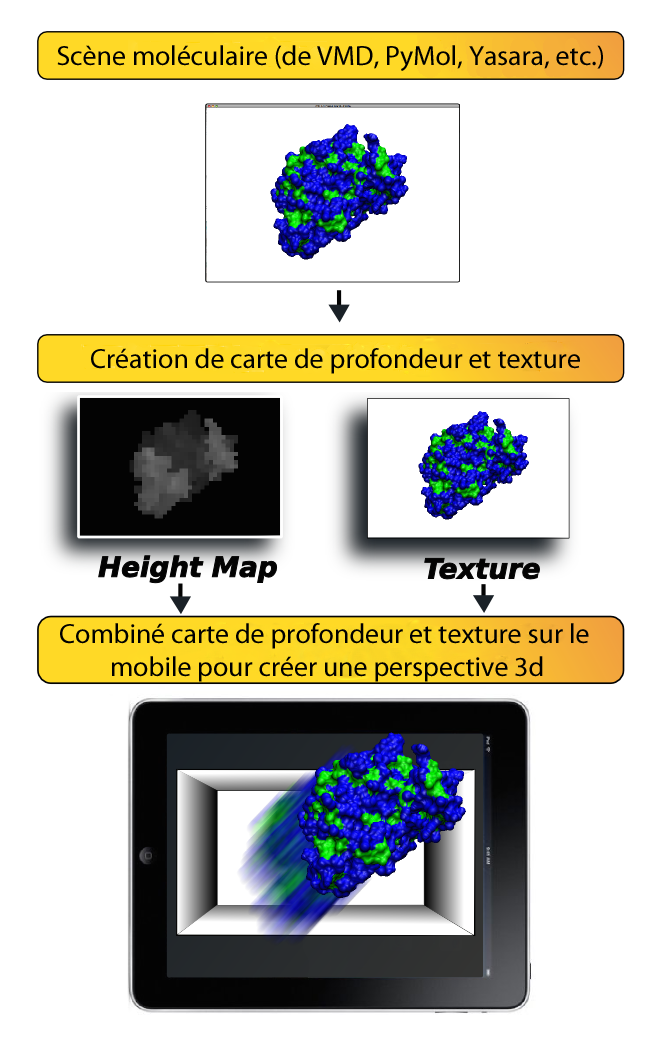
\includegraphics[width=.75\linewidth]{./figures/ch3/depthmol3d_process_edit}}
    \caption{}
  \label{Fig:depthmol3d_process}
  % \hspace{0.3cm}
\end{subfigure}
\begin{subfigure}{.5\textwidth}
  \centering
  {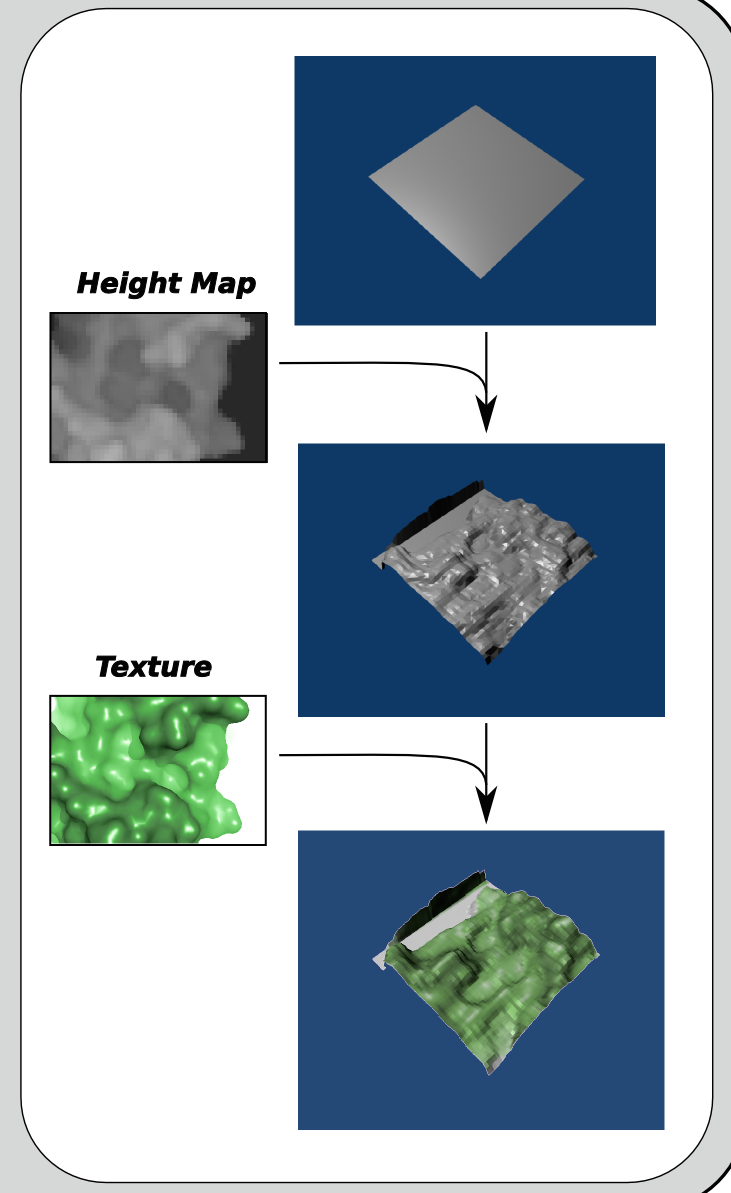
\includegraphics[width=.75\linewidth]{./figures/ch3/heightmap_texture_unity}}
    \caption{}
  \label{Fig:heightmap_texture_unity}
  % \hspace{0.3cm}
\end{subfigure}

\caption{{\it (a) Schéma du fonctionnement de notre application mobile. La première étape consiste à générer une carte de profondeur et une capture d'image de la scène moléculaire que l'on souhaite visualiser. Les deux images sont ensuite combinées au sein de l'application pour créer une perception 3d de la scène initiale.
(b) Le processus d'obtention d'un objet 3d à partir de 2 images. La première étape consiste à analyser la carte de profondeur pixel par pixel et de générer une surface aux dimensions identiques (à un facteur d'échelle près) dont la hauteur de chaque sommet sera corrélée avec le niveau de gris du pixel correspondant.}}
\end{figure}

\subsubsection{Ajouter la 3e dimension à une scène moléculaire}

Notre approche se base sur l'utilisation d'images 2d, beaucoup plus légères que des modèles 3d et permettant un certain degré de personnalisation de la part des utilisateurs. Indépendante de logiciels experts de visualisation, notre application ne nécessite qu'un périphérique mobile pour fonctionner et expérimenter l'effet 3d. Un nombre important de visualiseurs moléculaires peuvent être utilisés pour générer du contenu, VMD, Chimera, PyMol ou Yasara peuvent par exemple être utilisés pour générer ces scènes.

Deux images sont nécessaire pour parvenir à un effet 3d, une image de \textbf{texture} et une \textbf{carte de profondeur} (cf. Figure \ref{Fig:depthmol3d_process}). L'image de \textit{texture} est une capture simple de la scène 3d moléculaire alors que la \textit{carte de profondeur} ne possède elle que les informations de distance à l'écran pour l'image de texture. L'information de distance est codée grâce à un gradient de couleur grise. Ce gradient de gris correspond à la distance entre chaque point de la scène moléculaire 3d et l'écran. De ce fait, plus un objet est distant de la caméra (ou plus simplement de l'écran de la station de travail) et plus la couleur est sombre. Une fois que les deux images ont été générées, elles doivent être transférées sur le périphérique mobile où elles sont lues et traitées par notre application. Un navigateur de fichier intégré permet à l'utilisateur de trouver ses images et de les charger. 

Le traitement effectué par l'application permet tout d'abord de créer un objet 3d à partir de la carte de profondeur, objet dont la surface sera ensuite colorée par la texture associée (\ref{Fig:heightmap_texture_unity}). Le niveau de gris de chaque pixel de la carte de profondeur est ainsi interprété en tant que hauteur et correspond à un sommet de la surface 3d générée. Lorsque tous les pixels de la carte de profondeur ont été traités, les sommets de la surface 3d sont reliés par des segments afin de créer des objets continus qui seront ensuite colorés par la texture.

La scène 3d générée crée l'illusion d'une 3e dimension en ajoutant aux objets une impression d'espace et de profondeur qui s'étend loin derrière l'écran. Cela est rendu possible par les calculs permanents de la direction de vue basée sur l'orientation du périphérique, mesurée par un accéléromètre ou un gyroscope embarqués dans la majorité des périphériques mobiles d'aujourd'hui, amenant ainsi l'impression de regarder à l'intérieur d'une boîte qui s'étendrait derrière la surface d'écran de l'appareil.
Il est possible d'utiliser jusque 4 images (2 fois deux images contenant une carte de profondeur et une texture associée) afin de créer des scènes plus complexes possédant un arrière-plan et un premier-plan. Cette possibilité permet l'ajout d'informations complémentaires qui ne sont généralement pas présent au sein des visualiseur moléculaire d'où les scènes virtuelles sont extraites.

Plusieurs exemples sont fournis avec l'application et permettent à l'utilisateur d'appréhender les rendus 3d possibles et d'avoir une première prise en main des possibilités qu'offrent l'application. Les 5 exemples sont illustrés dans la Figure \ref{Fig:depthmol3d_exemple}.


\begin{figure}[h]
\begin{subfigure}{.5\textwidth}
  \centering
  {\includegraphics[width=.75\linewidth]{./figures/ch3/depthmol3d_exemple}}
    \caption{}
  \label{Fig:depthmol3d_exemple}
  % \hspace{0.3cm}
\end{subfigure}
\begin{subfigure}{.5\textwidth}
  \centering
  {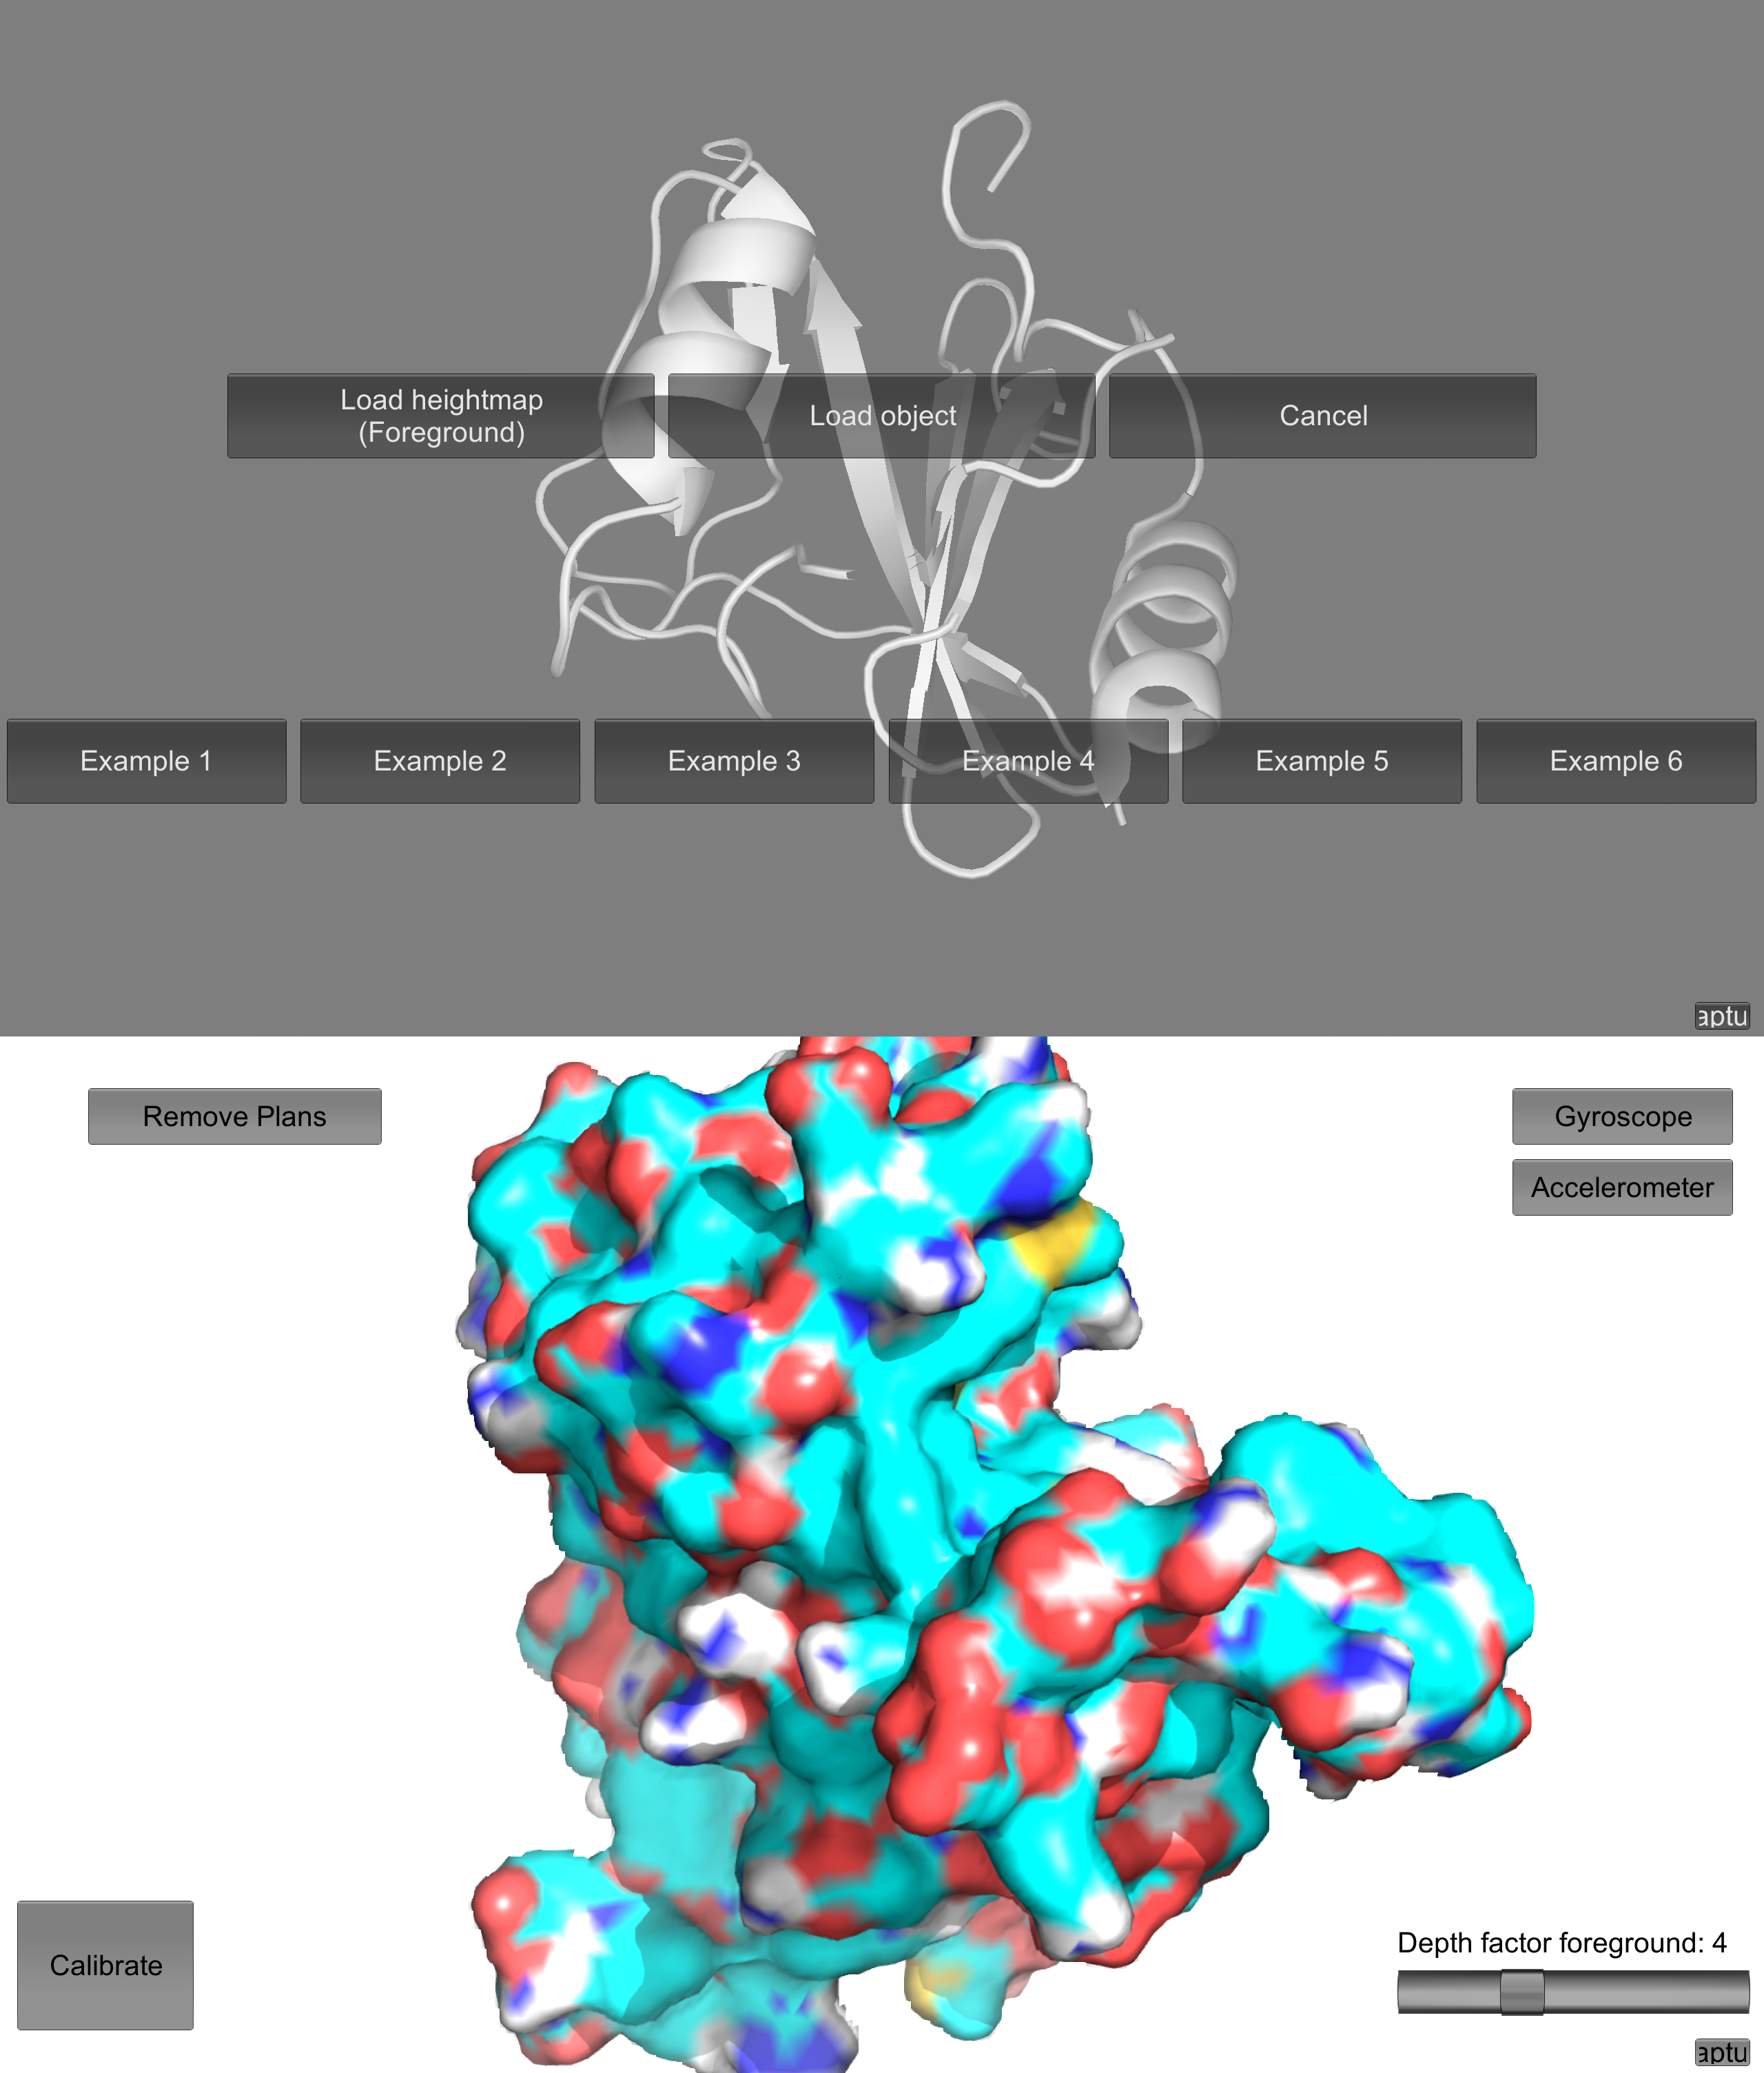
\includegraphics[width=.75\linewidth]{./figures/ch3/depthmol3d_screenshots}}
    \caption{}
  \label{Fig:depthmol3d_screenshots}
  % \hspace{0.3cm}
\end{subfigure}
\caption{{\it (a) Scènes moléculaires proposées par défaut en exemple au sein de l'application.
A. Visualisation d'une poche de liaison à la surface de GLIC (Ligand-Gated Ion Channel), une protéine transmembranaire responsable du passage des ions et des molécules d'eau à travers la membrane cellulaire. Scène extraite de VMD. B. Carte de basse résolution obtenue à partir de cryo-EM pour un filament d'actine. La position de la structure atomique dans l'enveloppe de basse résolution est en premier-plan alors que la carte électromagnétique est présentée en arrière-plan. Visualisation provenant de Chimera C. Couple verticale du modèle de la capside du virus Influenza A exposant la membrane externe et l'intérieur du virus. GraphiteLifeExplorer a été utilisé pour visualiser la coupure. D. Interaction entre une protéine SNARE et une membrane biologique lors d'une dynamique moléculaire (arrière-plan). Un graphe 3d rapportant le taux de courbure de la membrane est présenté en premier-plan. La surface 3d a été générée par Paraview (programme de visualisation scientifique) E. Scènes extraites d'un programme d'animation, MolecularMaya, dédié à la création de films scientifiques pour une audience large. Les scènes extraites mettent en avant deux virus au milieu de villosités à gauche et de multiples virus à droite.
(b) Captures d'écran provenant de l'application DepthMol3D et mettant en avant le menu principal de l'application permettant de charger une image ou un objet 3d (en haut) et une scène 3d type représentant la surface d'une protéine avec les différentes options de paramétrisation (en bas).}}
\end{figure}

\subsubsection{Explorer des modèles 3d de molécules}

Un deuxième mode de visualisation permet d'importer directement des fichiers d'objets 3d dans DepthMol3d. Avec ce type de données 3d, un seul fichier est nécessaire pour créer une perspective 3d complète de l'objet. Après importation, il est possible de manipuler l'objet, de le tourner, le déplacer en avant ou arrière. Cette visualisation se rapproche de ce qui peut se retrouver dans les visualiseurs moléculaires pour périphériques mobiles.
Pour aller plus loin dans l'immersion, l'utilisateur aura également la possibilité de changer l'échelle de la molécule et de plonger à l'intérieur et d'activer une visualisation plus interactive.
Il utilisera en effet son périphérique comme une fenêtre sur le monde virtuel et le manipulera en orientant le périphérique à la main et en l'utilisant comme une vue adaptative sur un monde virtuel présent tout autour de lui. Basés sur le gyroscope du périphérique, l'objet 3d est visualisable à 360 degrés mais à partir d'une position fixe. 

Pour une étape supplémentaire vers une immersion plus importante, un rendu stéréoscopique peut être effectué au sein d'un support de casque, à la manière de ce que proposent de nombreux acteurs de la RV aujourd'hui n'ayant pas franchi le pas de la conception de casques de RV mais fournissant des supports pour l'utilisation de smartphones (voir section \ref{dispositifs_RV}). Dans cette configuration, un simple mouvement de tête permet de regarder une zone différente de la molécule (voir Figure \ref{Fig:molexplorer_screenshot}). Cette approche est rendue possible par un mode stéréoscopique \textit{side-by-side} intégré au sein de l'application. 

\begin{figure}[h]
  \centering
  {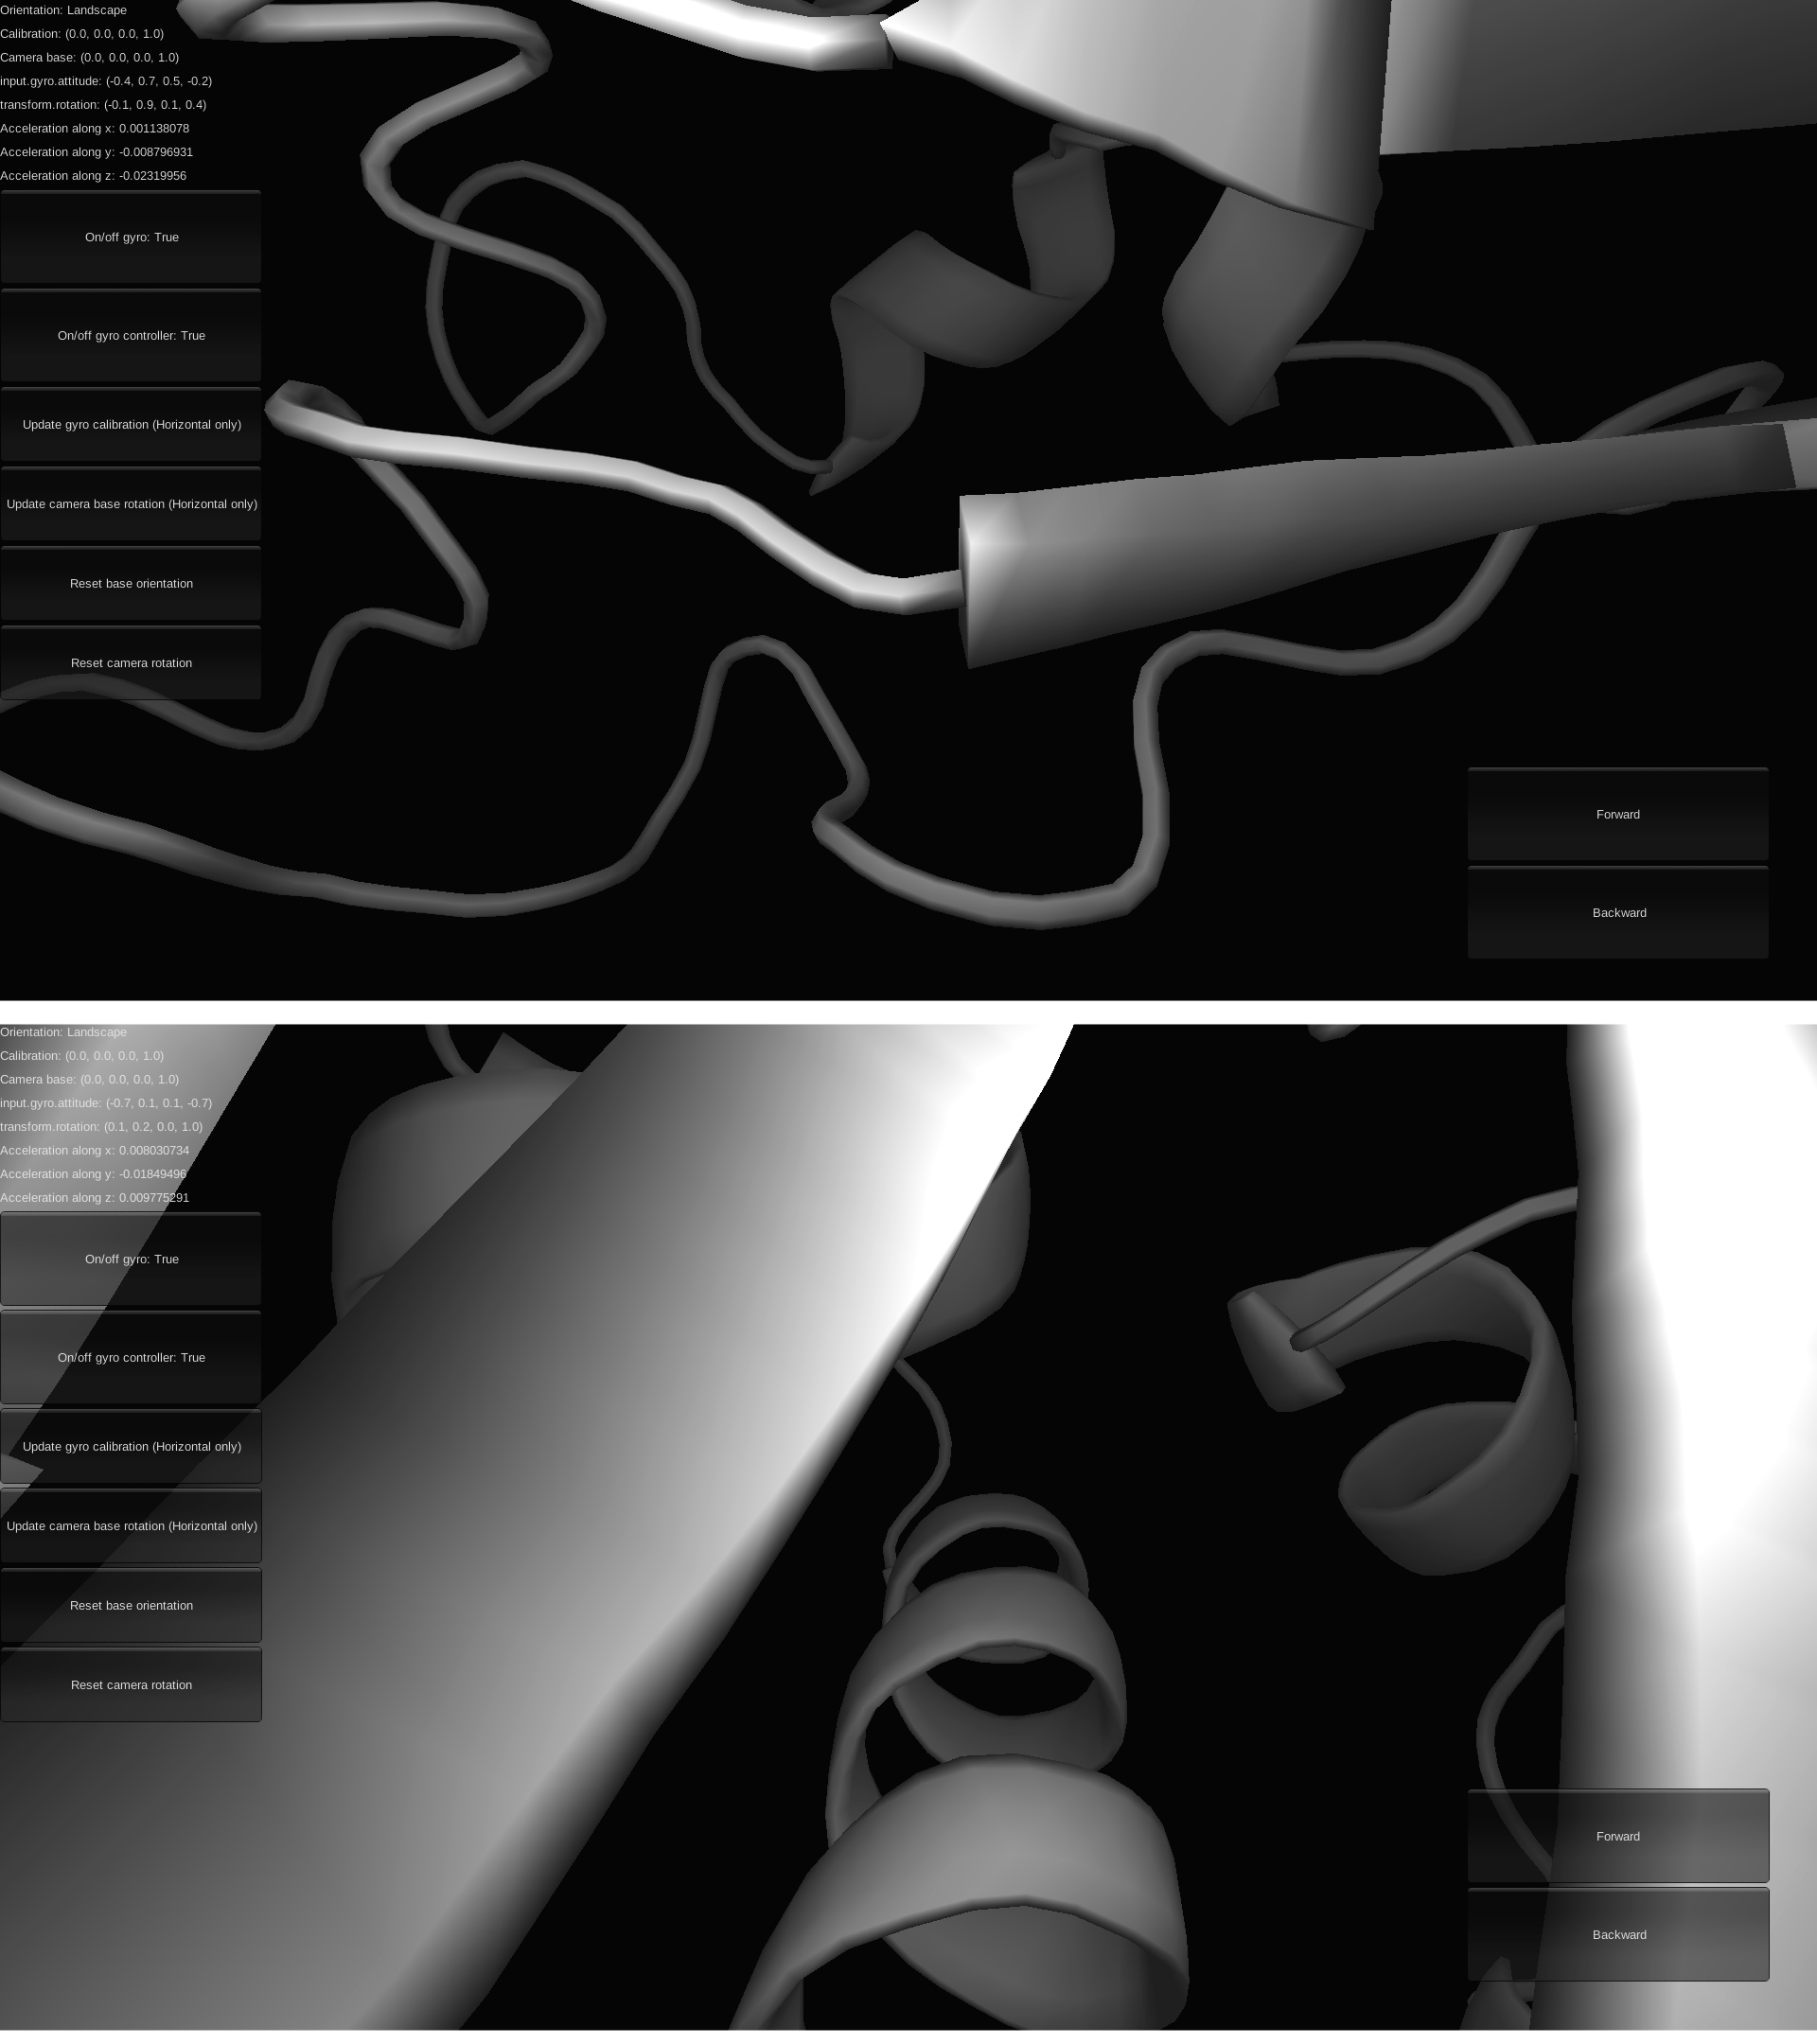
\includegraphics[width=.75\linewidth]{./figures/ch3/molexplorer_screenshot.png}}
    \caption{{\it Captures d'écran du mode d'exploration de modèles 3d au sein de l'application. La différence de point de vue entre les deux captures d'écran est le résultat d'une rotation du périphérique mobile tenu par l'utilisateur.}}
  \label{Fig:molexplorer_screenshot}
  \hspace{0.2cm}
\end{figure}

\subsubsection{Bilan}

La préparation des images utilisées au sein de l'application est relativement simple et rapide, des tutoriels sont en plus préparés pour aider les utilisateur à effectuer les actions nécessaires. Notre approche est indépendante de la plateforme de visualisation et la majorité des visualiseurs moléculaires permettant de générer des rendus graphiques de structures permettent de générer les images demandées. Il est également possible d'utiliser des outils génériques tels que Povray\footnote{\url{www.povray.com}} ou Paraview\footnote{\url{www.paraview.org}}. La création de vues complexes est rendue possible grâce à la notion d'arrière-plan et de premier-plan permettant ainsi de mettre en valeur certains aspects d'une scène virtuelle où la seule structure ne serait pas assez illustrative d'un phénomène particulier.

La performance de l'application permet son utilisation sur la plupart des smartphones et tablettes Android et iOS de moins de 5 ans et la quasi-intégralité des derniers smartphones/tablettes. DepthMol3D est gratuit et le code source est disponible à la demande.

Les limitations de notre application résident tout d'abord dans la résolution des écrans des périphériques et leurs angles de vue, tout deux limités par rapport aux stations de travail ou aux ordinateurs portables à cause de leur taille. Les cartes de profondeur sont pour le moment limitées à des résolutions assez basses et peuvent faire apparaître des artefacts quand les détails de la scènes sont trop fins. La limitation de la résolution des cartes de profondeur considérées dans l'application est due à la limitation technique du moteur Unity3D qui ne peut gérer des objets 3d de plus de 65536 sommets. Ceci implique donc l'utilisation de cartes de profondeur de 255*255 pixels de résolution au maximum. Il n'existe par contre aucune limitation dans la résolution de la texture tant que celle-ci est aux mêmes dimensions que la carte de profondeur. L'utilisation d'images 2d ne permet pas un contrôle total de l'objet 3d généré et sa manipulation dans l'espace. Notre mode d'importation d'objets 3d permet de pallier en partie cette limitation mais la performance du rendu est moindre, tout autant que la facilité de création de nouvelles structures.






